% Copyright 2004 by Till Tantau <tantau@users.sourceforge.net>.
%
% In principle, this file can be redistributed and/or modified under
% the terms of the GNU Public License, version 2.
%
% However, this file is supposed to be a template to be modified
% for your own needs. For this reason, if you use this file as a
% template and not specifically distribute it as part of a another
% package/program, I grant the extra permission to freely copy and
% modify this file as you see fit and even to delete this copyright
% notice. 

\documentclass{beamer}

% There are many different themes available for Beamer. A comprehensive
% list with examples is given here:
% http://deic.uab.es/~iblanes/beamer_gallery/index_by_theme.html
% You can uncomment the themes below if you would like to use a different
% one:
%\usetheme{AnnArbor}
%\usetheme{Antibes}
%\usetheme{Bergen}
%\usetheme{Berkeley}
%\usetheme{Berlin}
%\usetheme{Boadilla}
%\usetheme{boxes}
%\usetheme{CambridgeUS}
%\usetheme{Copenhagen}
%\usetheme{Darmstadt}
%\usetheme{default}
%\usetheme{Frankfurt}
%\usetheme{Goettingen}
%\usetheme{Hannover}
%\usetheme{Ilmenau}
%\usetheme{JuanLesPins}
%\usetheme{Luebeck}
\usetheme{Madrid}
%\usetheme{metropolis}
%\usetheme{Malmoe}
%\usetheme{Marburg}
%\usetheme{Montpellier}
%\usetheme{PaloAlto}
%\usetheme{Pittsburgh}
%\usetheme{Rochester}
%\usetheme{Singapore}
%\usetheme{Szeged}
%\usetheme{Warsaw}

%\usepackage{graphicx}
%\usepackage{placeins}
%%\usepackage{sidenotes}
%%\usepackage[a4paper,left=24.8mm,top=27.4mm,headsep=2\baselineskip,textwidth=107mm,
%%					marginparsep=8.2mm,marginparwidth=49.4mm,textheight=49\baselineskip,
%%					headheight=\baselineskip]{geometry} % tufte-handout definitions
%\usepackage[a4paper,
%left=22mm,top=27.4mm,
%headsep=2\baselineskip,
%textwidth=107mm, %110mm
%marginparsep=6.0mm, %4.0mm
%marginparwidth=70mm, %70mm
%textheight=52\baselineskip,
%headheight=\baselineskip]{geometry} % tufte-handout definitions

%=======Fonts and Language [XelateX only]=====
\usepackage{fontspec}
\usepackage{float}
\usepackage{morefloats}
\usepackage{polyglossia}
\usepackage{svg}

\setmainlanguage{greek}
\setotherlanguage{english}

\setmainfont{CF Jeckyl}
\newfontfamily\greekfont{CF Jeckyl}
\newfontfamily\greekfontsf{CF Jeckyl}
\newfontfamily\greekfonttt{CF Jeckyl}
%\setmainfont{Liberation Serif}
%\newfontfamily\greekfont{Liberation Serif}
%\newfontfamily\greekfontsf{Liberation Serif}
%\newfontfamily\greekfonttt{Liberation Serif}

%====Physics and Maths Symbols=============
\usepackage{amsmath}
\usepackage{amssymb}
\usepackage{xparse}
%\usepackage[arrowdel]{physicsrev} %Physics Packge (Revised)
\usepackage[arrowdel]{physics}
\usepackage[version=3]{mhchem} %Chemistry Symbols
\usepackage{wasysym} %Astronomical Symbols

\usepackage{siunitx} %Units
\usepackage{cancel}
\usepackage{multirow}
%=====Graphics=============
\usepackage{graphicx}
%\usepackage{caption}
\usepackage{lipsum, calc, needspace}
%\usepackage{subcaption}
\usepackage{textcomp}
%\usepackage{tikz}
\usepackage{scrextend}
%============================
\newlength\widthw
\setlength{\widthw}{\textwidth+\marginparsep+\marginparwidth}


\newlength{\fullwidthlen}
\setlength{\fullwidthlen}{\marginparwidth}
\addtolength{\fullwidthlen}{\marginparsep}

\newenvironment{fullwidth}{%
	\begin{adjustwidth*}{\ifthispageodd{-5cm}{-0cm}}{\ifthispageodd{-0cm}{-5cm}}%
	}{%
	\end{adjustwidth*}%
}

%======Other==============
\usepackage{multirow}
\usepackage{booktabs}
\usepackage{latexsym,graphicx}
\usepackage{todonotes}
%\usepackage{xcolor}
%\usepackage[some]{background}
%\usepackage{wrapfig}
%\usepackage{sidecap}
%\usepackage{lscape}
%\usepackage{rotating}
%\usepackage{geometry}

%===Bibliography======================
\usepackage[backend=biber,style=authoryear,citestyle=authoryear]{biblatex}
%\addbibresource{My Library.bib}

%=========Unit Declaration==========
\DeclareSIUnit \cm {\centi\meter}
\newcommand{\sm}{$M_{\odot}$}

\title{Αριθμητικές προσομοιώσεις νεφών σε γαλαξίες}
\author{Παπαχρήστου Μιχάλης}
%
%\numberwithin{equation}{subsection}
%\setsecnumdepth{chapter}
%\setcounter{secnumdepth}{3}
%\counterwithout{section}{chapter}
%\newcommand{\tabletodo}[3][]{\begin{minipage}{#2}\todo[inline,#1]{#3}\end{minipage}}
\sisetup{retain-unity-mantissa = false,range-phrase=\texttt{ έως },range-units = single,separate-uncertainty = true}

%\title{Presentation Title}

% A subtitle is optional and this may be deleted
%\subtitle{Optional Subtitle}

%\author{F.~Author\inst{1} \and S.~Another\inst{2}}
% - Give the names in the same order as the appear in the paper.
% - Use the \inst{?} command only if the authors have different
%   affiliation.

%\institute[Universities of Somewhere and Elsewhere] % (optional, but mostly needed)
%{
%  \inst{1}%
%  Department of Computer Science\\
%  University of Somewhere
%  \and
%  \inst{2}%
%  Department of Theoretical Philosophy\\
%  University of Elsewhere}
% - Use the \inst command only if there are several affiliations.
% - Keep it simple, no one is interested in your street address.

\date{28 Ιουνίου 2017}
% - Either use conference name or its abbreviation.
% - Not really informative to the audience, more for people (including
%   yourself) who are reading the slides online

%\subject{Theoretical Computer Science}
% This is only inserted into the PDF information catalog. Can be left
% out. 

% If you have a file called "university-logo-filename.xxx", where xxx
% is a graphic format that can be processed by latex or pdflatex,
% resp., then you can add a logo as follows:

% \pgfdeclareimage[height=0.5cm]{university-logo}{university-logo-filename}
% \logo{\pgfuseimage{university-logo}}

% Delete this, if you do not want the table of contents to pop up at
% the beginning of each subsection:
%\AtBeginSubsection[]
%{
%  \begin{frame}<beamer>{Outline}
%    \tableofcontents[currentsection,currentsubsection]
%  \end{frame}
%}

% Let's get started
\begin{document}

\begin{frame}
  \titlepage
\end{frame}

%\begin{frame}{Outline}
%  \tableofcontents
%  % You might wish to add the option [pausesections]
%\end{frame}

% Section and subsections will appear in the presentation overview
% and table of contents.
\section{Μεσοαστρική Ύλη}

%\subsection{First Subsection}

\begin{frame}{Μεσοαστρική Ύλη}{Τι υπάρχει μεταξύ των αστέρων?}
	Στο μεσοαστρικό χώρο έχουμε μια τεράστια ποσότητα ύλης υπό τη μορφή αερίου (99\%) και σκόνης (1\%). Στο γαλαξία μας η συνολική της μάζα είναι της τάξης των \SI{1e9}{ M_{\odot}}, ενώ η πυκνότητα της κυμαίνεται από \SIrange{1e-4}{1e6}{cm^{-3}}.
\begin{center}
	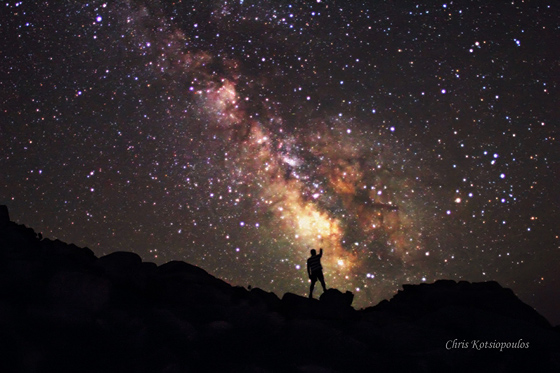
\includegraphics[width=0.8\linewidth]{Images/NightSkyPhotography04}
\end{center}
\end{frame}

\begin{frame}{Μεσοαστρικό αέριο}%{Φυσικά Χαρακτηριστικά}
\begin{center}
	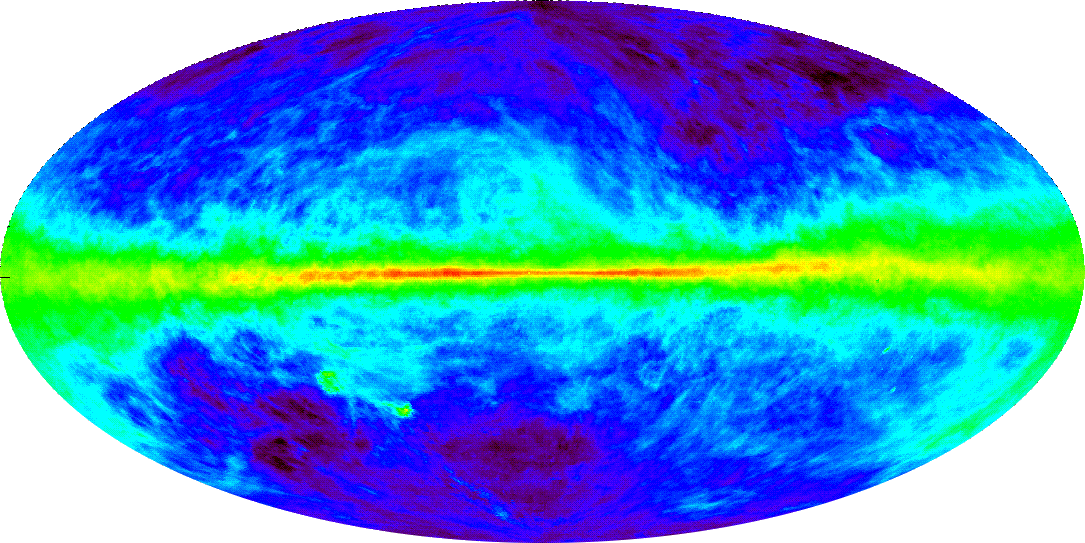
\includegraphics[width=1\linewidth]{../Document/Images/21}
\end{center}
		\begin{itemize}
			\item{(90\%) Υδρογόνο  \ce{(H)}, \ce{(HII)}, \ce{(H2)}}	
			\item{(9\%) Ήλιο }	
			\item{(1\%) Βαρύτερα στοιχεία  (\ce{C},\ce{O},\ce{Ne},\ce{Mg},\ce{Fe}, κ.α.) και άλλα μόρια (\ce{CO},\ce{CS}, κ.α.).}
		\end{itemize}

%		\begin{itemize}
%		\item{Υδρογόνο (\ce{HI}, \ce{HII}, \ce{H2} )}
%		\item{Ήλιο (\ce{HeI}, \ce{HeII})}
%		\item{Βαρύτερα στοιχεία (\ce{C}, \ce{O}, \ce{Ne}, \ce{Mg}, \ce{Fe})}
%		\item{Μόρια (\ce{CO}, \ce{CS}, και πολυπλοκότερα PAH)}
%		\item{Σκόνη}
%	\end{itemize}
\end{frame}

\begin{frame}{Μεσοαστρική Σκόνη}%{Χημική Σύσταση}
		\begin{itemize}
		\item{Αποτελείται κυρίως από άνθρακα και πυρίτιο σε ενώσεις με Υδρογόνο, Οξυγόνο, Μαγνήσιο και Σίδηρο}
			\item{Tο μέγεθος των κόκκων της σκόνης κυμαίνεται από \SI{0.01}{\micro\meter} έως \SI{1}{\micro\meter} ακολουθώντας μια κατανομή δύναμης όπου τα μικρότερα μεγέθη είναι πολυπληθέστερα από τα μεγαλύτερα.}
	\end{itemize}
	\begin{columns}
		\column{0.5\textwidth}
		\begin{center}
			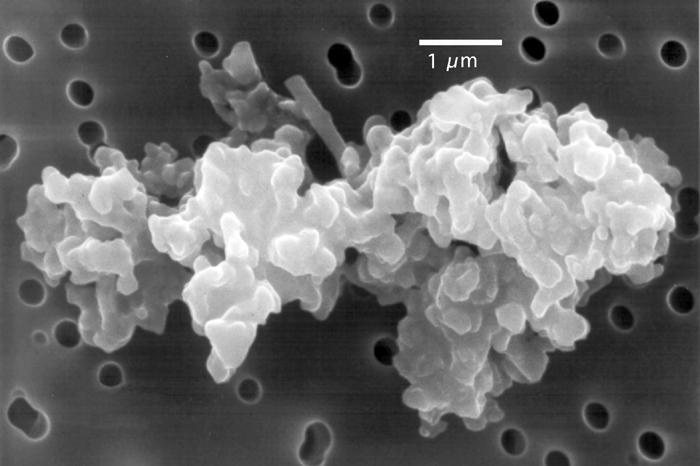
\includegraphics[width=1\linewidth]{Images/Porous_chondriteIDP}
		\end{center}
		
		\column{0.5\textwidth}
		\begin{itemize}
		%	\item{Αποτελείται κυρίως από άνθρακα και πυρίτιο σε ενώσεις με Υδρογόνο, Οξυγόνο, Μαγνήσιο και Σίδηρο}
		%	\item{Tο μέγεθος των κόκκων της σκόνης κυμαίνεται από \SI{0.01}{\micro\meter} έως \SI{1}{\micro\meter} ακολουθώντας μια κατανομή δύναμης όπου τα μικρότερα μεγέθη είναι πολυπληθέστερα από τα μεγαλύτερα.}
			\item{Παρατηρείται στις σπείρες του Γαλαξία μας (αλλά και σε άλλους γαλαξίες) με τη χαρακτηριστική μορφή τεράστιων σκοτεινών "δρόμων" λόγω της επισκότισης των όπισθεν αστέρων που προκύπτει από την απορρόφηση και σκέδαση του ορατού φωτός}
		\end{itemize}
	\end{columns}
\end{frame}

\begin{frame}{Μεσοαστρική Ύλη}{Κατηγοριοποίηση}
	\begin{description}
		\item[ψυχρή]{με θερμοκρασίες κάτω των \SI{100}{\kelvin},
			πυκνότητα \SIrange{30}{50}{cm^{-3}} και ποσοστό ιονισμού κάτω του 0.1\%, που αποτελείται από μοριακό και ατομικό αέριο Υδρογόνου και σκόνη}
		\item[θερμή]{με θερμοκρασίες της τάξης των \SIrange{1e3}{1e4}{K}, πυκνότητες \SI{0.3}{cm^{-3}}, που αποτελείται από ατομικό και ιονισμένο άεριο Υδρογόνο (ποσοστό ιονισμού 2-20\%)}
		\item[υπέρθερμη]{οφείλεται σε κρουστικά κύματα εκρήξεων supernova και αστρικών ανέμων με θερμοκρασίες τάξης \SI{1e6}{K} και πυκνότητες μικρότερες των \SI{0.01}{cm^{-3}}.}
	\end{description}
\end{frame}

\begin{frame}{Εκπομπή \ce{H\alpha}}
\begin{center}
	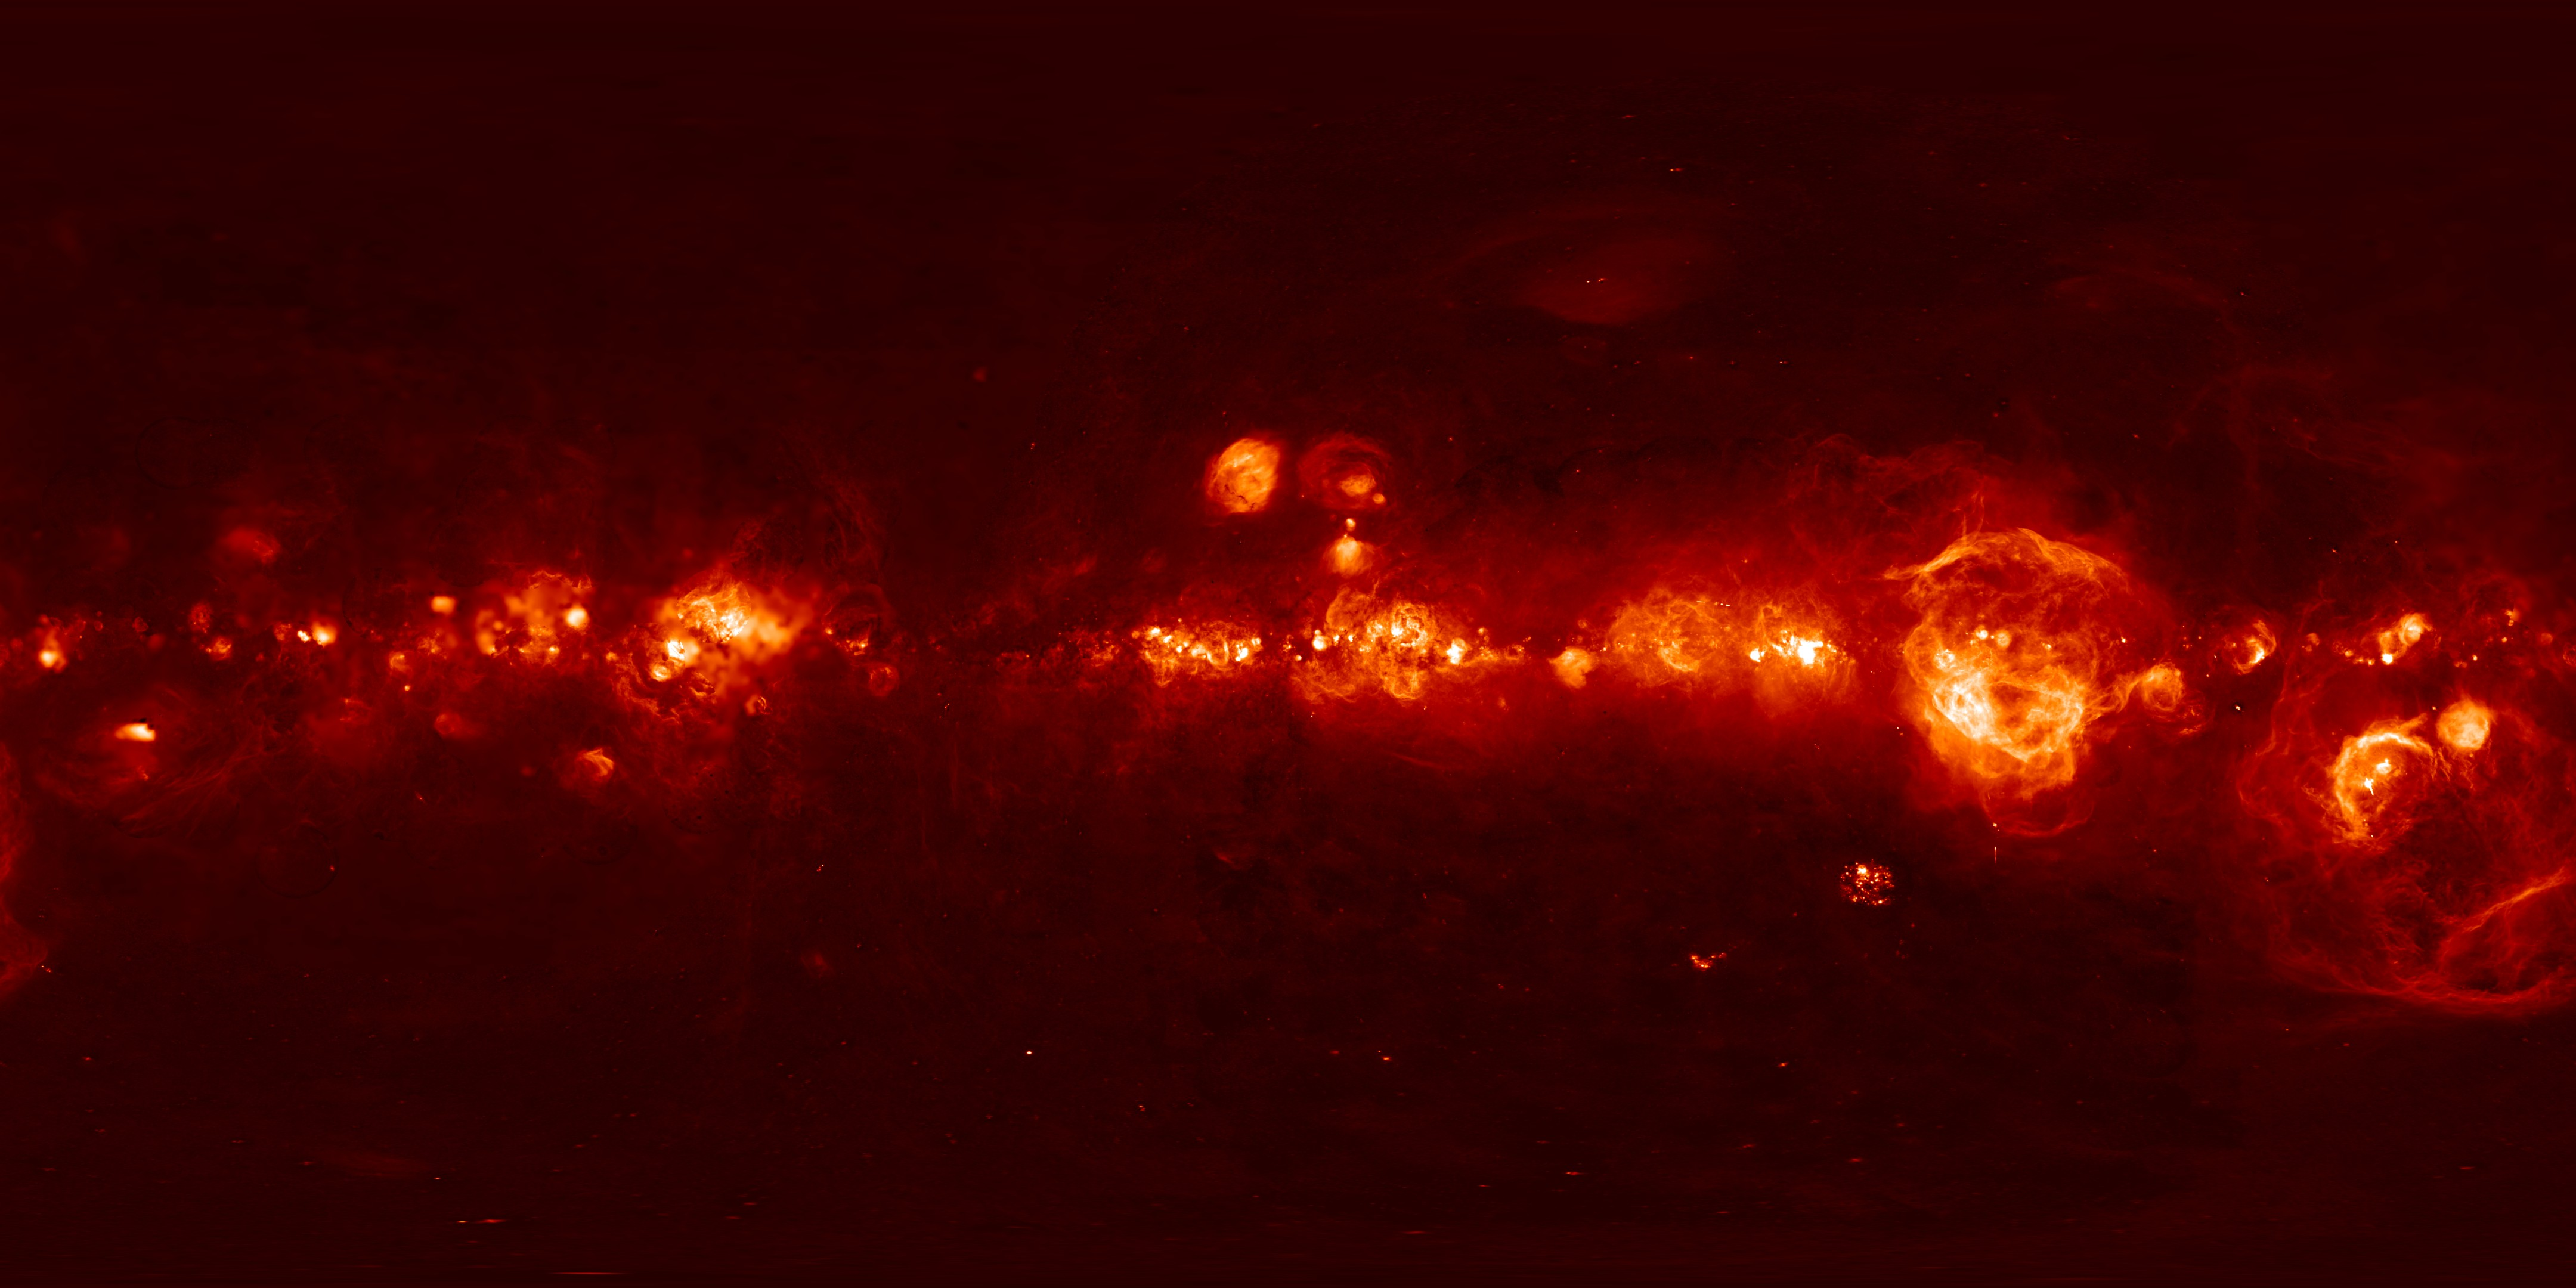
\includegraphics[width=1\linewidth]{../Document/Images/Ha}
\end{center}
	Εκπομπή Ha (\SI{656.28}{nm}) από συνδυασμό τριών διαφορετικών παρατηρήσεων (WHAM - VTSS - SHASSA)
	%Η εκπομπή Ha  προέρχεται από την επανασύνδεση ιονισμένων ατόμων υδρογόνου κοντά σε θερμούς αστέρες O και B (\ce{HII} Regions).
\end{frame}

\begin{frame}{Εκπομπή \ce{CO}}
\begin{center}
	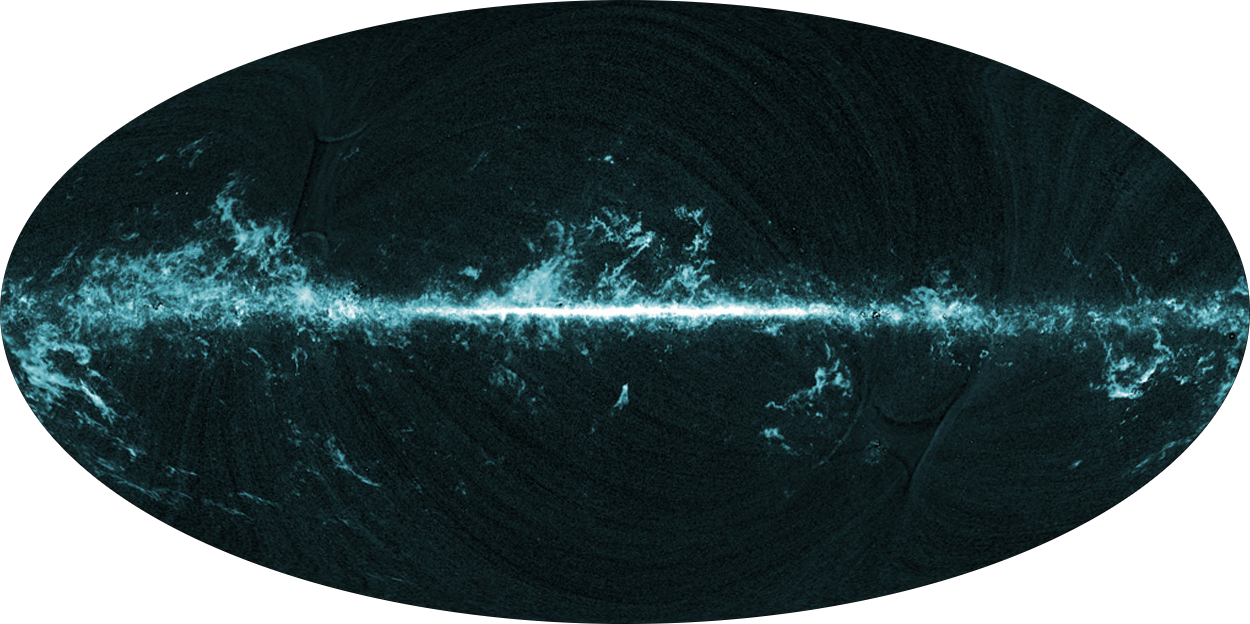
\includegraphics[width=1\linewidth]{../Document/Images/CO}
\end{center}
 Εκπομπή \ce{CO} που αντιστοιχεί σε θερμοκρασία \SI{5.5}{K} και αποδίδει ένα ραδιοφωνικό φωτόνιο στα \SI{2.6}{mm}.
\end{frame}

\begin{frame}{Μεσοαστρική Ύλη}{Φυσικά Χαρακτηριστικά - Σύνοψη}
\begin{table}
	\begin{tabular}{p{2.5cm} c  c  c }
		\toprule
		\multirow{2}{*}{Κατηγορία}  & Θερμοκρασία & Πυκνότητα   \\ 
		& \si{(K)} & \si{(cm^{-1})}  \\
		\midrule
		Μοριακά Νέφη & 10-50 & \num{>1e3} \\
		Ψυχρά Νέφη \ce{HI}  & \num{100} & \num{30} \\
		Θερμό \ce{HI}  & \num{1e3} & \num{0.1} \\
		Θερμό \ce{HII}  & \num{1e4} & \num{1e-2} \\
		Περιοχές \ce{HII} &  \num{1e4} & \num{>100} \\
		Υπέρθερμο Ιονισμένο αέριο &  \numrange{1e6}{1e7} & \num{1e-3} \\
		\bottomrule
	\end{tabular}
\end{table}
\end{frame}

\subsection{Μοριακά Νέφη}

% You can reveal the parts of a slide one at a time
% with the \pause command:
\begin{frame}{Μοριακά Νέφη}
	\begin{itemize}
		\item{Περιοχές όπου η ψυχρή μεσοαστρική ύλη έχει πυκνότητες ικανοποιητικά μεγαλύτερες από τη μέση πυκνότητα του μεσοαστρικού υλικού ώστε η ιδιοβαρύτητα του νέφους να παίζει σημαντικό ρόλο στη δυναμική του.}
		\item{Κατά τη βαρυτική κατάρρευση το ΜΝ κατακρημνίζεται σε όλο και πιο συμπυκνωμένες δομές έως ότου η πυκνότητα και η μάζα σε μια τέτοια περιοχή είναι αρκετή ώστε να γεννηθούν νέοι αστέρες. }
		\item{Αποτελούνται κυρίως από μοριακό Υδρογόνο \ce{H2} το οποίο μπορεί να δημιουργηθεί χάρη στις συνθήκες θερμοκρασίας - πίεσης και την ύπαρξη της σκόνης}
	\end{itemize} 
	
%  \begin{itemize}
%  \item {
%    First item.
%    \pause % The slide will pause after showing the first item
%  }
%  \item {   
%    Second item.
%  }
%  % You can also specify when the content should appear
%  % by using <n->:
%  \item<3-> {
%    Third item.
%  }
%  \item<4-> {
%    Fourth item.
%  }
%  % or you can use the \uncover command to reveal general
%  % content (not just \items):
%  \item<5-> {
%    Fifth item. \uncover<6->{Extra text in the fifth item.}
%  }
%  \end{itemize}
\end{frame}

\begin{frame}{Μοριακά Νέφη}{Κατηγοριοποίηση}
\begin{table}
	\caption{Χαρακτηριστικά και διαφορετικοί τύποι Μοριακών Νεφών}
	\begin{tabular}{l c c c c}
		\toprule
		\multirow{2}{*}{Κατηγορία} & Μέση ακτίνα &  Θερμοκρασία & Πυκνότητα \ce{H2} & Μάζα \\ 
		& \si{(pc)} & \si{(K)} & \si{(cm^{-3})} & \si{(M_\odot)} \\
		\midrule
		Γιγαντιαίο Μοριακό Νέφος & \num{20} & \num{15} & \num{100} & \num{1e5} \\
		Μοριακό Νέφος & $5$ & $10$ & $300$ & $10^4$\\
		clump & $2$ & $10$ & $10^3$ & $10^3$\\
		Πυρήνας Νέφους & $0.08$ & $10$ & $10^5$ & $10$\\
		\bottomrule
	\end{tabular}
\end{table}
\end{frame}

\begin{frame}{Ενεργειακή ισορροπία στη Μεσοαστρική Ύλη}
Ξεκινάμε από τον πρώτο νόμο τις θερμοδυναμικής:
\begin{equation}
dE = \bar{d}Q - dW
\end{equation}

Θεωρώντας τη καταστατική εξίσωση ιδανικού αερίου ο ρυθμός θέρμανσης/ψύξης ανά μονάδα όγκου είναι:
\begin{equation}
\Delta =\frac{1}{V} \frac{dQ}{dt} =n\frac{d}{dt}\left(\frac{3}{2}kT \right)-kT\frac{dn}{dt}
\end{equation}

 Ορίζουμε τις συναρτήσεις ψύξης (cooling function) $\Lambda$ και θέρμανσης (heating function) $\Gamma$ ώστε
\begin{equation}
\Delta = \Gamma -\Lambda
\end{equation}
\end{frame}

\begin{frame}{Μηχανισμοί Θέρμανσης}{Κοσμική Ακτινοβολία (1)}
Κατά την αλληλεπίδραση ενός πρωτονίου της κοσμικής ακτινοβολίας με το μοριακό υδρογόνο
\begin{equation}
\ce{p^+ +H2 -> H2 ^+ +e^- +p^+}
\end{equation}

Ενώ στη περίπτωση της αλληλεπίδρασης της κοσμικής ακτινοβολίας με ουδέτερο Υδρογόνο ο ιονισμός πραγματοποιείται μέσω της:
\begin{equation}
\ce{p^+ + H -> H^+ + e^- + p^+}
\end{equation}
Και στις δύο περιπτώσεις το ηλεκτρόνιο που διαφεύγει μπορεί είτε να ιονίσει περαιτέρω το μοριακό αέριο μέσω της
\begin{equation}
\ce{e^- + H2 -> H2^+ + e^- + e^-}
\end{equation}
η οποία δεν προσδίδει θέρμανση αλλά εμπλουτίζει το χώρο με περισσότερο ενεργητικά ηλεκτρόνια ή να θερμάνει τελικά το αέριο μέσω της διάσπασης του μορίου
\begin{equation}
\ce{e^- + H2 -> H + H + e^-}
\end{equation} 


%Κάνοντας το λεπτομερή υπολογισμό μέσω του δικτύου όλων τα πιθανών σεναρίων βρίσκουμε ότι η ενεργειακή ενέργεια ανά ιονισμό είναι $\Delta E (\ce{H2}) = \SI{7}{eV}$.
\end{frame}


\begin{frame}{Μηχανισμοί Θέρμανσης}{Κοσμική Ακτινοβολία (2)}

Ο ρυθμός θέρμανσης γενικά δίνεται από τη
\begin{equation}
\Gamma _\mathtt{CR} (\ce{X}) =\zeta (\ce{X})n_{\ce{X}} \Delta E (\ce{X})
\end{equation}
όπου η ενεργεία ανά ιονισμό ($\Delta E (\ce{X})$) βρίσκεται από το λεπτομερή υπολογισμό μέσω του δικτύου όλων τα πιθανών σεναρίων ενώ οι ρυθμοί ιονισμού ($\zeta (\ce{X})$) βρίσκονται από παρατηρησιακά δεδομένα.
\begin{block}{Ρυθμοί Θέρμανσης λόγω κοσμική ακτινοβολίας}
 \begin{align}
\Gamma _\mathtt{CR} (\ce{HI}) &= \num{1.6e-25} \left( \frac{n_{\ce{HI}}}{\SI{1e3}{cm^{-3}}} \right) \qq{(\si{erg.cm^{-3}.s^{-1}})} \\
\Gamma _\mathtt{CR} (\ce{H2}) &= \num{3.2e-25} \left( \frac{n_{\ce{H2}}}{\SI{1e3}{cm^{-3}}} \right) \qq{(\si{erg.cm^{-3}.s^{-1}})} 
\end{align}
\end{block}

\end{frame}

\begin{frame}{Μηχανισμοί Θέρμανσης}{Διάχυτη Ακτινοβολία (1)}
	\begin{center}
			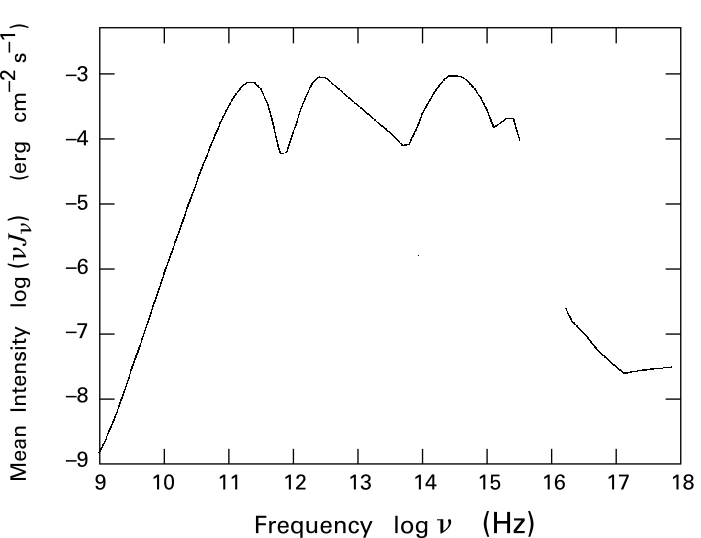
\includegraphics[width=0.7\linewidth]{../Document/Images/interstellarradiation}
	\end{center}
\end{frame}

\begin{frame}{Μηχανισμοί Θέρμανσης}{Διάχυτη Ακτινοβολία (2)}
	\begin{description}
		\item[κοσμικό υπόβαθρο (\SI{1e11.3}{Hz})]{Τα φωτόνια του κοσμικού υποβάθρου θερμαίνουν τα μοριακά νέφη διεγείροντας τις χαμηλότερες περιστροφικές ενεργειακές στάθμες του \ce{CO}.}
		\item[εκπομπή σκόνης (\SI{1e12.4}{Hz})]{Τα μοριακά νέφη είναι διάφανα σε αυτή την ακτινοβολία}
		\item[εκπομπή αστέρων (\SI{1e14.5}{Hz})]{Διέγερση ηλεκτρόνιων που δεν καταφέρνουν να δραπετεύσουν από τους κόκκους σκόνης και τους θερμαίνουν}
		 \begin{block}{Θέρμανση των κόκκων σκόνης}
		 	\begin{equation}
		 	\Gamma _\mathtt{d} = \num{3.2e-21} \left( \frac{n_{\ce{H}}}{\SI{1e3}{cm^{-3}}} \right) \qq{(\si{erg.cm^{-3}.s^{-1}})} 
		 	\end{equation} 	
		 \end{block}	
	\end{description}
\end{frame}


\begin{frame}{Μηχανισμοί Θέρμανσης}{Διάχυτη Ακτινοβολία (3)}
	\begin{description}
		\item[υπεριώδες (\SI{1e15.3}{Hz})]{Ιονισμός του ατομικού άνθρακα (\ce{CI}) ($\frac{n_{\ce{CI}}}{n_{\ce{H}}} =\num{3e-4}$, ενέργεια ιονισμού στα \SI{1e11.2}{eV}), ιονισμός και απελευθέρωση ηλεκτρονίων από τους κόκκους σκόνης}
		\end{description}
		\begin{block}{Θέρμανση μέσω ιονισμού του άνθρακα}
			  \begin{equation}
			\Gamma _\mathtt{IR} (\ce{CI}) = \num{6.41e-23} \left( \frac{n_{\ce{H}}}{\SI{1e3}{cm^{-3}}} \right) \qq{(\si{erg.cm^{-3}.s^{-1}})} 
			\end{equation}
		\end{block}	
			\begin{block}{Θέρμανση μέσω ιονισμού των ηλεκτρονίων των κόκκων σκόνης}
\begin{equation}
\Gamma _\mathtt{PE} = \num{4.8e-23} \left( \frac{n_{\ce{H}}}{\SI{1e3}{cm^{-3}}} \right) \qq{(\si{erg.cm^{-3}.s^{-1}})} 
\end{equation}
	\end{block}	
\end{frame}

%\begin{frame}{Μηχανισμοί Θέρμανσης}{Άλλοι μηχανισμοί}
%	
%\end{frame}

\begin{frame}{Μηχανισμοί Ψύξης}{Ψύξη μέσω αλληλεπίδρασης ηλεκτρονίου - ιόντος}
	\begin{columns}
		\column{0.35\textwidth}
\begin{center}
	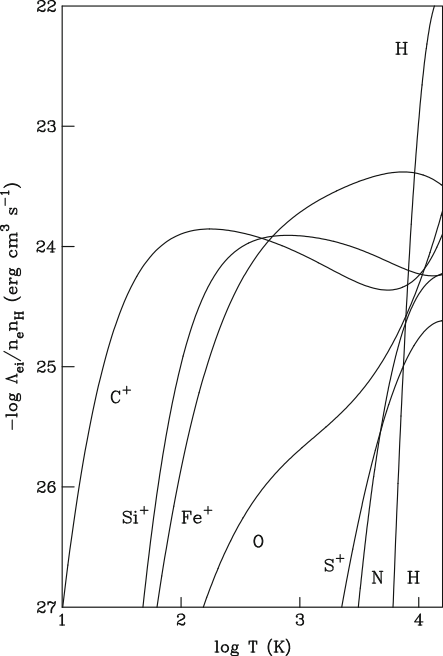
\includegraphics[height=0.7\textheight]{../Document/Images/eiCoolingFunction}
\end{center}

		\column{0.65\textwidth}
		\begin{itemize}
			\item{Σημαντικός μηχανισμός στο Μεσοαστρικό αέριο λόγω μεγαλύτερου ιονισμού}
		\end{itemize}
		\begin{equation}
		\Lambda _\mathtt{ei}=\num{8.6e-6} n_\mathtt{e} n_\mathtt{iu}T^{-1/2} e^{-E_\mathtt{ul}/k_b T}\frac{E_\mathtt{ul}\Omega (\mathtt{u,l})}{g_\mathtt{u}} \qq{(\si{erg.cm^{-3}.s^{-1}})} 
		\end{equation}
	\end{columns}
\end{frame}

\begin{frame}{Μηχανισμοί Ψύξης}{Ψύξη μέσω αλληλεπίδρασης Υδρογόνου - ιόντος}
	\begin{description}
		\item[$n_{\ce{H}}<n_\mathtt{crit}=A_\mathtt{ul}/\gamma _\mathtt{ul}$]{	
			\begin{equation}
			\Lambda _\mathtt{H.ul} = n_\mathtt{l} n_{\ce{H}} \gamma _\mathtt{ul} \Delta E _\mathtt{ul} = \frac{g_\mathtt{u}}{g_\mathtt{l}} n_\mathtt{l} n_{\ce{H}} \gamma _\mathtt{ul} \Delta E_\mathtt{ul} e^{-T_o/T}
			\end{equation}}
		\item[$n_{\ce{H}}<n_\mathtt{crit}=A_\mathtt{ul}/\gamma _\mathtt{ul}$]{LTE:
		\begin{equation}
		\Lambda _\mathtt{H.ul} = n_\mathtt{l}  A _\mathtt{ul} \Delta E _\mathtt{ul} = \frac{g_\mathtt{u}}{g_\mathtt{l}} n_\mathtt{l} A _\mathtt{ul} \Delta E_\mathtt{ul} e^{-T_o/T}
		\end{equation}
	}
	\end{description}

\begin{block}{Κύριοι Ψύκτες}
			\begin{equation}
		\Lambda _{\ce{H - OI}}=\num{3.2e-22} \left( \frac{n_{\ce{H}}}{\SI{1e3}{cm^{-3}}} \right)^2 e^{\left( \frac{\SI{-230}{K}}{T} \right) } \qq{(\si{erg.cm^{-3}.s^{-1}})} 
		\end{equation}
		\begin{equation}
	\Lambda _{\ce{H - CII}}=\num{4.8e-21} \left( \frac{n_{\ce{H}}}{\SI{1e3}{cm^{-3}}} \right)^2 e^{\left( \frac{\SI{-92}{K}}{T} \right) } \qq{(\si{erg.cm^{-3}.s^{-1}})} 
	\end{equation}
\end{block}
\end{frame}

\begin{frame}{Μηχανισμοί Ψύξης}{Ψύξη μορίων και σκόνης}
	\begin{itemize}
		\item{Στις χαμηλές θερμοκρασίες (<\SI{100}{K}) κύριος ψύκτης είναι το \ce{CO}.}
		\item{Πολύπλοκος μηχανισμός καθώς σε μεγάλο βαθμό οι εκπομπές είναι οπτικά πυκνές.}
	\end{itemize}
	\begin{equation}
	\Lambda _{\ce{CO}}=\num{8e-24} \frac{(J^*+1)^5}{\theta (2J^*+1)} e^{-\frac{(J^*+1)(J^*+2)}{2\theta}}
	\left( \frac{n_{\ce{H}}}{\SI{1e3}{cm^{-3}}} \right)  \qq{(\si{erg.cm^{-3}.s^{-1}})} 
	\end{equation}

	\begin{itemize}
		\item{Οι κόκκοι σκόνης θερμαίνονται εκτός από την απορρόφηση στο υπεριώδες και οπτικό και μέσω συγκρούσεων με τα μόρια και άτομα του νέφους}
		\item{θεωρώντας τους σαν  μέλαν σώμα με τυπική θερμοκρασία \SI{30}{K} εκπέμπουν με μέγιστο στα \SI{100}{\mu m}}
	\end{itemize}
	\begin{equation}
	\Lambda _{\ce{CO}}=\num{1.6e-22} \left( \frac{n_{\ce{H}}}{\SI{1e3}{cm^{-3}}} \right) 
	\left( \frac{T_d}{\SI{10}{K}} \right)^6  \qq{(\si{erg.cm^{-3}.s^{-1}})} 
	\end{equation}
\end{frame}

\begin{frame}{Αριθμητικές υδροδυναμικές προσομοιώσεις}{Εξισώσεις Διατήρησης}
	Οι εξισώσεις διατήρησης είναι χρονοεξαρτώμενα συστήματα μερικών διαφορικών εξισώσεων με τη γενική μορφή:
	\begin{equation}
	\label{eq:hyperbolicconservation}
	\pdv{t} \bar{q}(x,t) + \pdv{x} \bar{f}(\bar{q}(x,t)) = 0 
	\end{equation}
	
	αποτελούν τη γενικότερη (μη γραμμική) μορφή των γραμμικών υπερβολικών εξισώσεων με μορφή:
	\begin{equation}
	\label{eq:linearhyperbolic}
	\pdv{\bar{q}}{t} +  \mathbf{A}\pdv{\bar{q}}{x}  = 0 
	\end{equation}
	όπου $\mathbf{A}$ ένας τετραγωνικός διαγωνοποιήσιμος πίνακας με πραγματικές ιδιοτιμές.
	
Η (\ref{eq:linearhyperbolic}) επιδέχεται αντίστοιχες λύσεις με την απλή κυματική εξίσωση
	\begin{equation}
	\label{eq:simple_advection}
	\pdv{q}{t} +  u\pdv{q}{x}  = 0 
	\end{equation}
	η οποία έχει σαν λύση τη κυματική λύση D'Alembert
	\begin{equation}
	q(x,t)=q(x-ut,0)
	\end{equation}
\end{frame}


\begin{frame}{Αριθμητικές υδροδυναμικές προσομοιώσεις}{Εξισώσεις Διατήρησης (2)}
	Στη μη-γραμμική περίπτωση το σύστημα λέγεται υπερβολικό αν ο ιακωβιανός πίνακας $\mathbf{J}(q)$ με στοιχεία $(i,j)$ τα $\pdv{f_i}{g_j}$ είναι αντίστοιχα διαγωνοποιήσιμος με πραγματικές ιδιοτιμές.
	
	Τότε μπορούμε να γράψουμε το σύστημα των μη-γραμμικών εξίσωσεων στη μορφή:
	\begin{equation}
	\pdv{\bar{q}}{t} + \mathbf{J}(\bar{q}) \pdv{\bar{q}}{x} = 0 
	\end{equation}
\end{frame}

\begin{frame}{Αριθμητικές υδροδυναμικές προσομοιώσεις}{εξισώσεις Euler (1)}
	Οι εξισώσεις euler είναι ένα σύστημα μη-γραμμικών υπερβολικών μερικών διαφορικών εξισώσεων που περιγράφουν ένα ρευστό χωρίς ιξώδες και θερμική αγωγιμότητα.
	\begin{block}{Εξισώσεις Euler}
		\begin{align}
		&\pdv{\rho}{t} + \div(\rho \vec{u})=0 \label{eq:MassHD} && 
		\texttt{Διατήρηση Μάζας} \\
		&\pdv{t}(\rho  \vec{u})+\div(\rho  \vec{u}  \vec{u} +P)=0 && 
		\texttt{Διατήρηση Ορμής} \label{eq:MomentumHD} \\
		&\pdv{E}{t}+\div((E+P)\vec{u})=0 \label{eq:EnergyHD} && 
		\texttt{Διατήρηση Ενέργειας}
		\end{align}
	\end{block}
με $E=\frac{P}{\gamma -1} +\frac{1}{2}\rho u^2$
\end{frame}
	
\begin{frame}{Αριθμητικές υδροδυναμικές προσομοιώσεις}{εξισώσεις Euler (2)}
	Σύμφωνα με τα προηγούμενα μπορούμε να γράψουμε το σύστημα στη μορφή \ref{eq:hyperbolicconservation}:
	\begin{equation}
	\pdv{t} \bar{q}(\vec{x},t) + \div\mathbf{f}(\bar{q}(\vec{x},t)) = 0 
	\end{equation}
	όπου 
	\begin{equation}
	\bar{q}(\vec{x},t)=\mqty(\rho \\ 
	\rho  \vec{u} \\
	E)
	=
	\mqty(q_1 \\ 
	q_2 \\
	q_3)
	\end{equation}
	και
	\begin{equation}
	\mathbf{f}(\bar{q}) = \mqty(\rho \vec{u} \\ 
	\rho \vec{u}\vec{u} + P \\
	\vec{u}(E+P))
	= \mqty(q_2 \\ 
	\frac{q_2 ^2}{q_1} +P(\bar{q}) \\
	\frac{q_2}{q_1} (q_3+P(\bar{q})))
	\end{equation}
	όπου $P(\bar{q}) $ η καταστατική εξίσωση. 
\end{frame}
	
\begin{frame}{Αριθμητικές υδροδυναμικές προσομοιώσεις}{Μέθοδος πεπερασμένων διαφορών}
	Διακριτοποιούμε το χώρο $\Delta x=\Delta y = h$ και στο χρόνο $\Delta t=k$ τότε η προσεγγιστική τιμή στη θέση $(x_\mathrm{i},y_\mathrm{j})=(x_0+\mathrm{i}h,y_0+\mathrm{j}h)$ και στο χρόνο $t_\mathrm{n}=t_0+\mathrm{n}k$ θα είναι:
	\begin{equation}
	Q_{\mathrm{ij}}^\mathrm{n }\simeq q(x_\mathrm{i},y_\mathrm{j},t_\mathrm{n})
	\end{equation}
	Οπότε η μερική διαφορική εξίσωση της μορφής
	\begin{equation}
	\pdv{q}{t}+u\pdv{q}{x}=0
	\end{equation} 
	με αρχικές συνθήκες $q_i^0$ θα έχει λύση στο κελί με συντεταγμένες $\mathrm{ijn}$:
	\begin{equation}
	Q_{\mathrm{i}}^\mathrm{n+1} = Q_{\mathrm{i}}^\mathrm{n} -\frac{k}{h} u \left( Q_\mathrm{i}^\mathrm{n} - Q_\mathrm{i-1}^\mathrm{n} \right)
	\end{equation} 
	
	Αντίστοιχα στη περίπτωση ενός συστήματος εξισώσεων η λύση θα ήταν
	\begin{equation}
	Q_{\mathrm{i}}^\mathrm{n+1} = Q_{\mathrm{i}}^\mathrm{n} -\frac{k}{h} \mathbf{Α} \left( Q_\mathrm{i}^\mathrm{n} - Q_\mathrm{i-1}^\mathrm{n} \right)
	\end{equation} 
	με τον πίνακα $\mathbf{Α}$ να έχει θετικές ιδιοτιμές. 
\end{frame}


\begin{frame}{Αριθμητικές υδροδυναμικές προσομοιώσεις}{Μέθοδος Πεπερασμένων Όγκων}
	Αντί για τη προσεγγιστική τιμή $Q_{\mathrm{i}}^\mathrm{n+1}$ της $q(x_\mathrm{i},t_\mathrm{n+1})$ σε ένα συγκεκριμένο σημείο θα ορίσουμε μια νέα αντίστοιχη τιμή για τη μέση τιμή της ποσότητας σε κάθε ένα διάστημα $C_\mathrm{i}=[x_\mathrm{i},x_\mathrm{i+1}]$ του χώρου μας με $x_\mathrm{i}=x_0+(i-1)h$. 
	
	Άρα τώρα η τιμή $Q_{\mathrm{i}}^\mathrm{n}$ θα προσεγγίζει την μέση τιμή στο $\mathrm{i}$ διάστημα τη χρονική στιγμή $t_\mathrm{n}$
	\begin{equation}
	Q_{\mathrm{i}}^\mathrm{n} \simeq \frac{1}{h} \int _{C_\mathrm{i}} q(x,t_\mathrm{n})dx
	\end{equation}
	Αν πάρουμε την ολοκληρωτική μορφή του νόμου διατήρησης σε ένα κελί η εξέλιξη στο χρόνο θα είναι
\begin{equation}
\label{eq:FVM}
Q_{\mathrm{i}}^\mathrm{n+1} = Q_{\mathrm{i}}^\mathrm{n} - \frac{k}{h}\left(F_{\mathrm{i+1}}^\mathrm{n}-F_{\mathrm{i}}^\mathrm{n} \right) 
\end{equation}
όπου 
\begin{equation}
F_{\mathrm{i}}^\mathrm{n} \simeq \frac{1}{k}\int_{t_\mathrm{n}}^{t_\mathrm{n}}f(q(x_\mathrm{i},t))dt 
\end{equation}
\end{frame}

\begin{frame}{Αριθμητικές υδροδυναμικές προσομοιώσεις}{Μέθοδος Πεπερασμένων Όγκων (2)}
	Είναι λογικό να υποθέσουμε ότι η ροή στο σύνορο μεταξύ δύο κελιών εξαρτάται από τις τιμές των ποσοτήτων σε αυτά τα δύο κελιά, δηλαδή
	
	\begin{equation}
	F_{\mathrm{i}}^\mathrm{n} = F\left( Q_{\mathrm{i-1}}^\mathrm{n} ,Q_{\mathrm{i}}^\mathrm{n} \right) 
	\end{equation}
	άρα αν γνωρίζουμε αυτή τη συνάρτηση ροής τότε μπορούμε να υπολογίσουμε την εξέλιξη στο χρόνο της μέσης τιμής του κάθε κελιού
	\begin{equation}
	Q_{\mathrm{i}}^\mathrm{n+1} = Q_{\mathrm{i}}^\mathrm{n} - \frac{k}{h}\left(
	F\left( Q_{\mathrm{i}}^\mathrm{n} ,Q_{\mathrm{i+1}}^\mathrm{n} \right)-
	F\left( Q_{\mathrm{i-1}}^\mathrm{n} ,Q_{\mathrm{i}}^\mathrm{n} \right)
	\right) 
	\end{equation} 
\end{frame}

\begin{frame}{Αριθμητικές υδροδυναμικές προσομοιώσεις}{Πρόβλημα Riemann}
\begin{columns}
	\column{0.5\textwidth}
	\begin{center}
		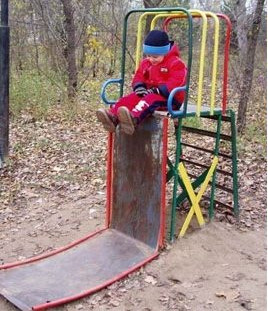
\includegraphics[width=1\linewidth]{Images/riemann-problem}
	\end{center}
	\column{0.5\textwidth}
	Το πρόβλημα Riemann είναι η επίλυση του νόμου διατήρησης της μορφής
	\begin{equation}
	\pdv{\bar{q}}{t}+\pdv{f(\bar{q})}{x}=0
	\end{equation}
	με αρχικές συνθήκες όπου υπάρχει μια ασυνέχεια:
	\begin{equation}
	\bar{q}(x,0)=
	\begin{cases}
	\bar{q}_\mathrm{L} &\qq{για} x<0 \\
	\bar{q}_\mathrm{R} &\qq{για} x>0 
	\end{cases}
	\end{equation}
\end{columns}
\end{frame}

\begin{frame}{Αριθμητικές υδροδυναμικές προσομοιώσεις}{Γραμμικό πρόβλημα Riemann}
	Η επίλυση του προβλήματος Riemann στη γραμμική περίπτωση του νόμου διατήρησης, δηλαδή στο σύστημα
	\begin{equation}
	\pdv{\bar{q}}{t} +  \mathbf{A}\pdv{\bar{q}}{x}  = 0 
	\end{equation}
	βασίζεται στο μετασχηματισμό των ποσοτήτων $\bar{q}$ στις λεγόμενες χαρακτηριστικές μεταβλητές $\bar{\xi}=\mathbf{R}^{-1}\bar{q}$ όπου $\mathbf{R}=(\bar{r}_1,\bar{r}_2,\cdots \bar{r}_m)$ είναι ο πίνακας των ιδιοανυσμάτων του πίνακα $\mathbf{A}$, ενώ με $\bar{\Lambda}=\mathtt{diag}(\lambda _1,\lambda _2,\cdots \lambda _m)$ ορίζουμε το διαγώνιο πίνακα των ιδιοτιμών.
	
	Οι εξισώσεις τότε γράφονται:
	\begin{equation}
	\pdv{\bar{\xi}}{t} + \bar{\Lambda} \div\bar{\xi} =0
	\end{equation} 
	δηλαδή σαν ένα διαχωρισμένο σύστημα εξισώσεων με λύσεις:
	\begin{equation}
	\label{eq:xi_solution}
	\xi_p  = \xi_p(x-\lambda _p t,0) 
	\end{equation}
	Οι $p$ χαρακτηριστικές καμπύλες δηλαδή καθορίζονται από τις ιδιοτιμές $\lambda _p$.
\end{frame}


\begin{frame}{Αριθμητικές υδροδυναμικές προσομοιώσεις}{Γραμμικό πρόβλημα Riemann (2)}
	
\begin{columns}
	\column{0.6\textwidth}
	\begin{center}
		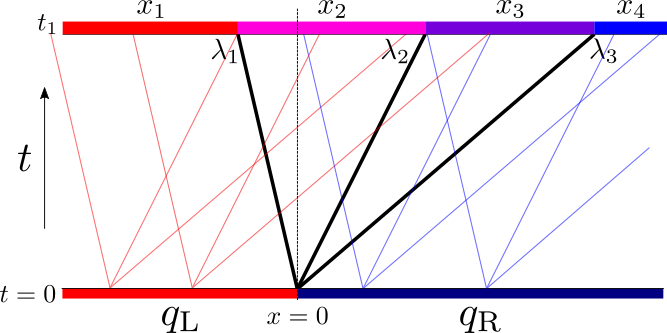
\includegraphics[width=1\linewidth]{../Document/Images/reimannlinear}
	\end{center}
	\column{0.4\textwidth}
Οι λύσεις σε κάθε σημείο του χώρου καθορίζονται απόλυτα από τις $p$ χαρακτηριστικές ιδιοτιμές $\lambda _p$ έτσι ώστε η τελική λύση για κάθε σημείο $x$ να είναι ο γραμμικός συνδυασμός των περιοχών που επηρεάζουν αυτό το σημείο, δηλαδή
\begin{align*}
q(x_1,t_1)&=\xi _1 ^L r_1 +\xi _2 ^L r_2 + \xi _3 ^L r_3 \\
q(x_2,t_1)&=\xi _1 ^R r_1 +\xi _2 ^L r_2 + \xi _3 ^L r_3 \\
q(x_3,t_1)&=\xi _1 ^R r_1 +\xi _2 ^R r_2 + \xi _3 ^L r_3 \\
q(x_4,t_1)&=\xi _1 ^R r_1 +\xi _2 ^R r_2 + \xi _3 ^R r_3 
\end{align*} 
\end{columns}
\end{frame}

\begin{frame}{Αριθμητικές υδροδυναμικές προσομοιώσεις}{Μη Γραμμικό πρόβλημα Riemann}
	Η συνάρτηση ροής της διατηρούμενης ποσότητας εξαρτάται πια από την ίδια τη ποσότητα, δηλαδή:
	\begin{equation}
	\pdv{t} \bar{q}(x,t) + \pdv{x} \bar{f}(\bar{q}(x,t)) = 0 
	\end{equation}
	
	Για ομαλές λύσεις μπορούμε να μετασχηματίσουμε το παραπάνω σύστημα μέσω της ιακωβιανής $\mathbf{J} =\mathbf{f}'$
	\begin{equation}
	\pdv{t} \bar{q}(x,t) + \mathbf{J}(q(x,t)) \pdv{q}{x}  = 0 
	\end{equation}
	
	\begin{columns}
		\column{0.5\textwidth}
			\begin{center}
				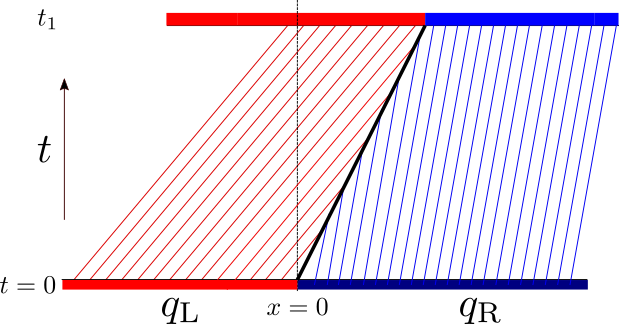
\includegraphics[width=0.9\linewidth]{../Document/Images/shockwave}
			\end{center}
		\column{0.5\textwidth}	
			\begin{center}
				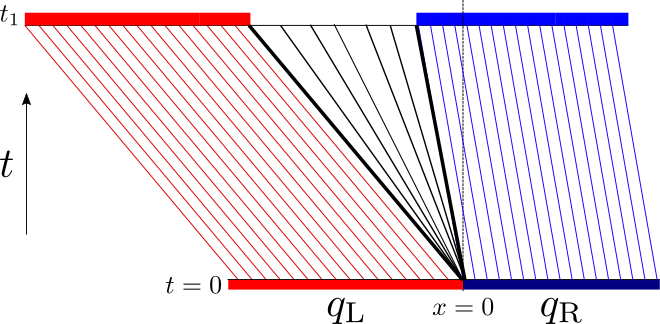
\includegraphics[width=0.9\linewidth]{../Document/Images/rarefuctionwave}
			\end{center}
	\end{columns}
\end{frame}	


\begin{frame}{Προσομοίωση Cooling}{Ορισμός του Test Problem}
	
\begin{columns}
	\column{0.5\textwidth}
	\begin{center}
		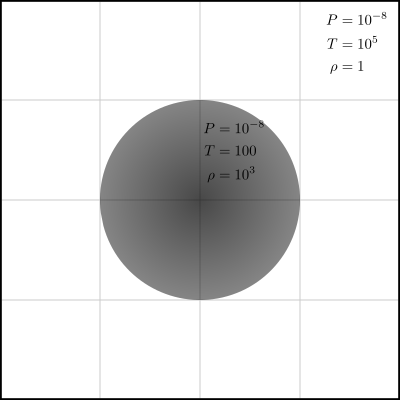
\includegraphics[width=1\linewidth]{../Document/Images/rect4578}
	\end{center}
	
	\column{0.5\textwidth}
	\begin{itemize}
		\item{Σφαιρικό, ομοιογενές νέφος που βρίσκεται αρχικά σε ισορροπία πίεσης με το διαγαλαξιακό χώρο.}
		\item{Χρονικό διάστημα \SI{~8}{Myrs} η οποία εκτιμήθηκε από τη σχέση $c_s/L_\mathtt{cloud}$ όπου $c_s$ η ταχύτητα του ήχου και $L_\mathtt{cloud}$ η ακτίνα του νέφους. }
	\end{itemize}
\end{columns}
\end{frame}

\begin{frame}{Σφαιρικό νέφος μέσα στο ISM}{No Cooling}
\begin{center}
	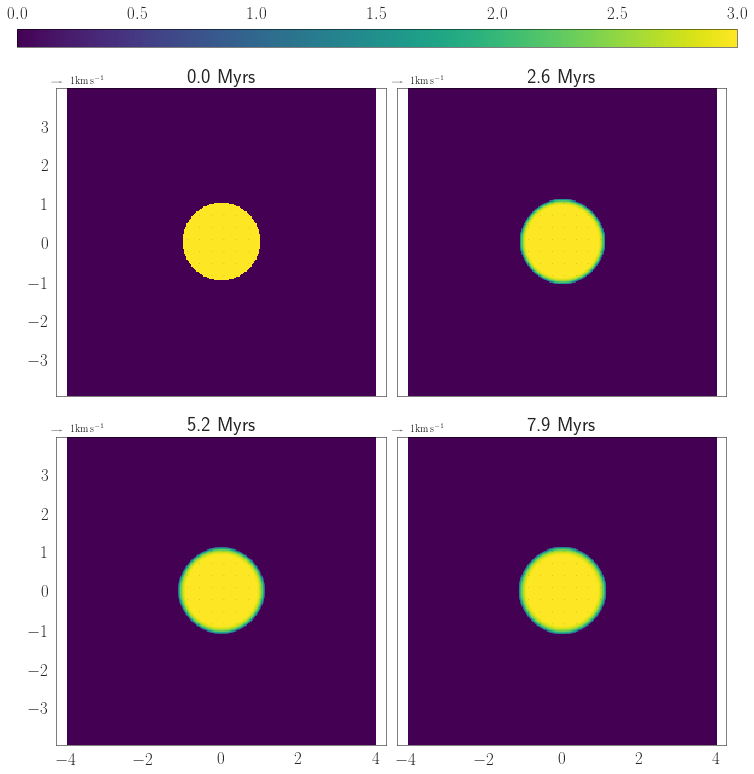
\includegraphics[width=1\linewidth]{../Document/DataImages/NoCoolingRHOquad}
\end{center}
\end{frame}

\begin{frame}{Σφαιρικό νέφος μέσα στο ISM}{Tabulated Cooling}
%		Το οπτικό βάθος για ένα φωτόνιο που εκπέμπεται (στο οπτικό ) μέσα στο νέφος είναι:
%	\begin{equation}
%	\tau = nL\sigma _T\simeq \num{6.65e-3}
%	\end{equation}
%	
\begin{columns}
	\column{0.5\textwidth}
	\begin{center}
		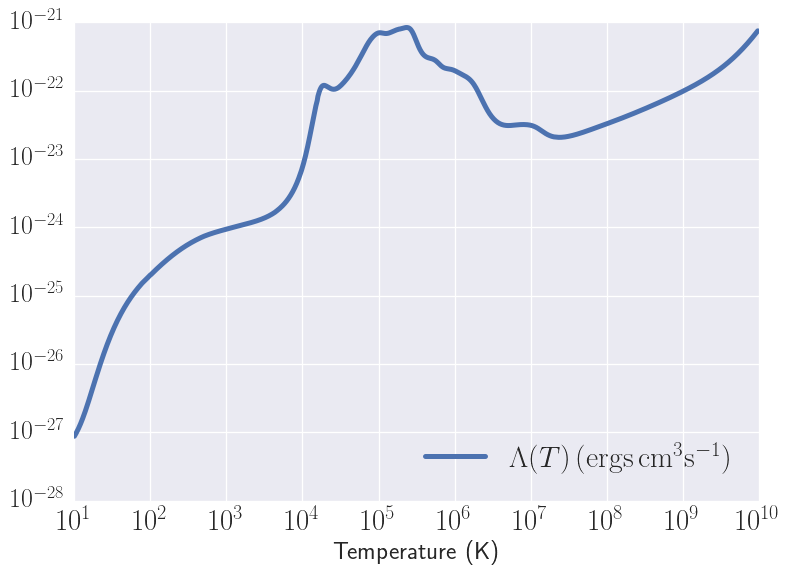
\includegraphics[width=1\linewidth]{../Document/Images/LambdaT}
	\end{center}
	\column{0.5\textwidth}
	\begin{itemize}
		\item{Για θερμοκρασίες χαμηλότερες των \SI{1e4}{K} η ψύξη προέρχεται από μοριακές εκπομπές (\ce{H2},\ce{CO} κλπ)}
		\item{Για θερμοκρασίες \SIrange{1e4}{1e7}{K} οι γραμμές εκπομπής των μετάλλων κυριαρχούν}
		\item{Για θερμοκρασίες ανώτερες των \SI{1e7}{K} κυριαρχεί η ακτινοβολία bremmstrahlung}
	\end{itemize}
\end{columns}
\end{frame}

\begin{frame}{Σφαιρικό νέφος μέσα στο ISM}{Tabulated Cooling}
Χρονική κλίμακα ψύξης του νέφους:
	\begin{equation}
	\tau _c =\frac{ \rho e} {n^2 \Lambda (T)}=
	\frac{ \frac{3}{2}k_b T} {n \Lambda (T)} 
	\simeq 10^8\si{s}\simeq \SI{3}{yrs} << \SI{1e5}{yrs}
	\end{equation}
	H αντίστοιχη χρονική κλίμακα και για το εξωτερικό του νέφους βρίσκουμε περίπου \SI{600}{yrs}. 
	
\begin{center}
	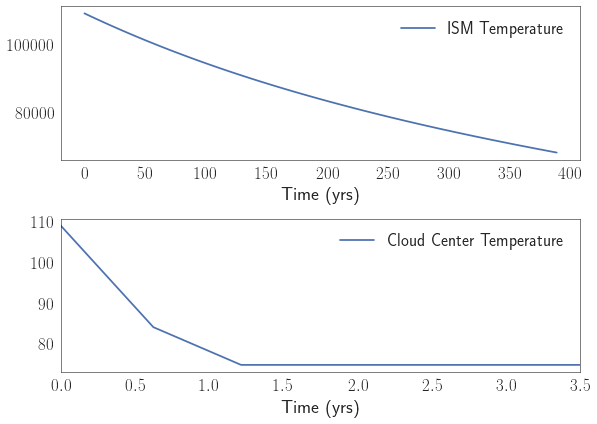
\includegraphics[width=0.55\linewidth]{../Document/DataImages/TabCoolingTMPcenterISM}
\end{center}
\end{frame}

\begin{frame}{Σφαιρικό νέφος μέσα στο ISM}{Tabulated Cooling}
\begin{columns}
	\column{0.55\textwidth}
	\begin{center}
		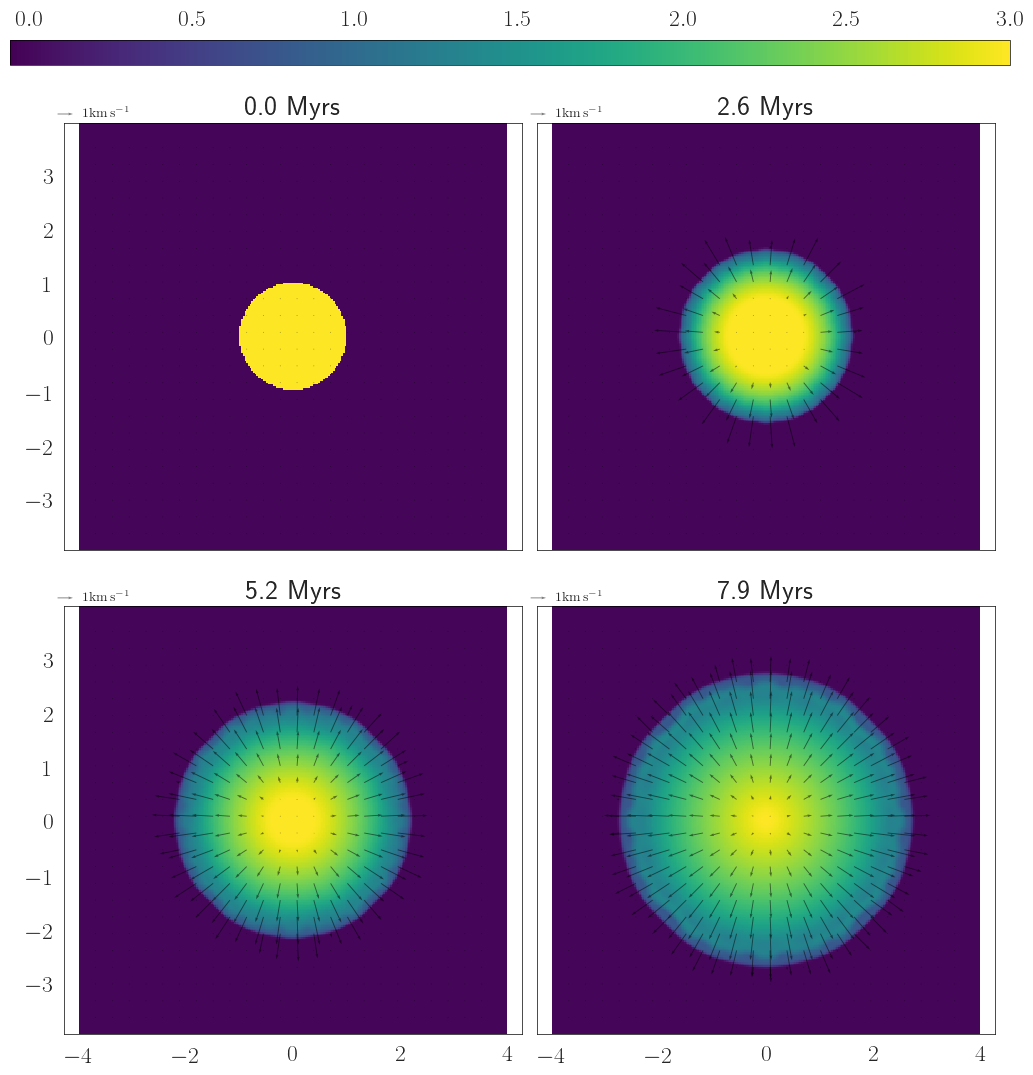
\includegraphics[width=1\linewidth]{../Document/DataImages/TabCoolingRHOquad}
	\end{center}
	\column{0.45\textwidth}
	\begin{itemize}
		\item{Το αέριο στο εσωτερικό του νέφους κρυώνει γρηγορότερα απ' ότι στο εξωτερικό περιβάλλον με συνέπεια η πίεση $P \sim \rho T$ να μικραίνει γρηγορότερα στο εσωτερικό (εφόσον αρχικά είναι ίδια παντού). Αυτή η διαφορά πίεσης δημιουργεί μια  δύναμη η οποία θα έπρεπε να επιταχύνει το αέριο προς το εσωτερικό του. }
	\end{itemize}
\end{columns}
\end{frame}

\begin{frame}{Σφαιρικό νέφος μέσα στο ISM}{Tabulated Cooling}
	\begin{columns}
		\column{0.5\textwidth}
			\begin{center}
				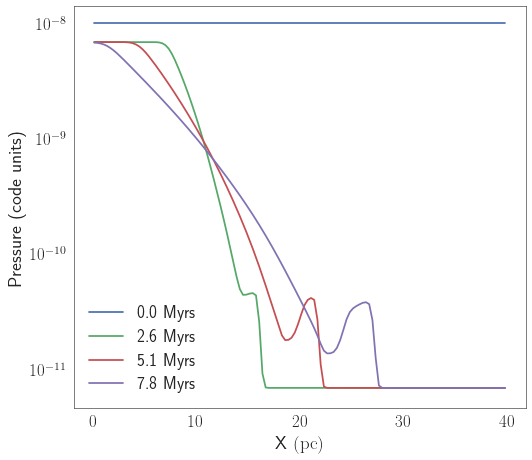
\includegraphics[width=1\linewidth]{../Document/DataImages/TabCoolingPRSprofile}
			\end{center}
		\column{0.5\textwidth}
			\begin{center}
				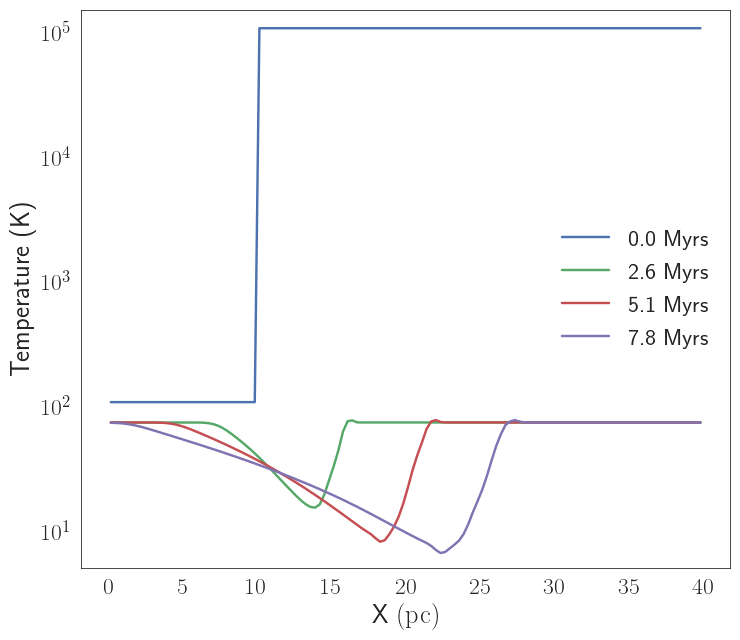
\includegraphics[width=1\linewidth]{../Document/DataImages/TabCoolingTMPprofile}
			\end{center}
	\end{columns}
\end{frame}

\begin{frame}{Σφαιρικό νέφος μέσα στο ISM}{Tabulated Cooling/ Small time scale}
	\begin{columns}
		\column{0.5\textwidth}
			\begin{center}
				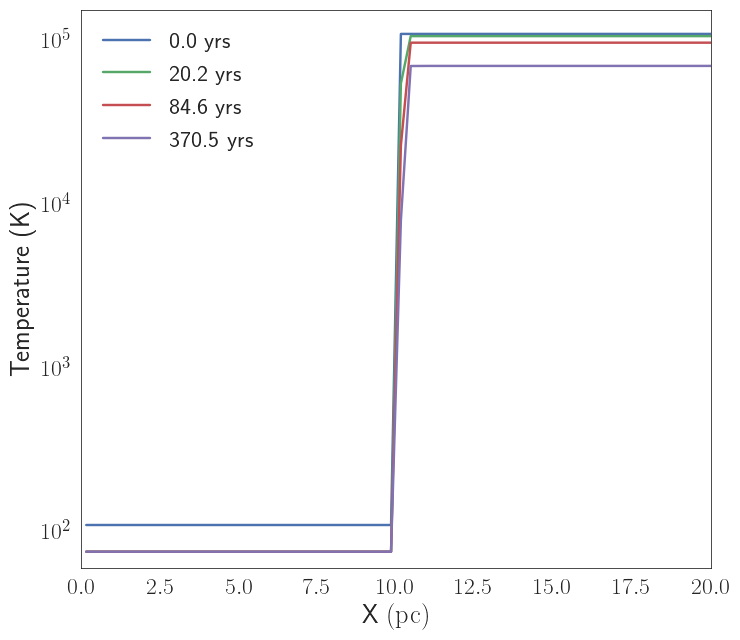
\includegraphics[width=1\linewidth]{../Document/DataImages/TabCoolingTMPprofile-micro}
			\end{center}
		\column{0.5\textwidth}
			\begin{center}
				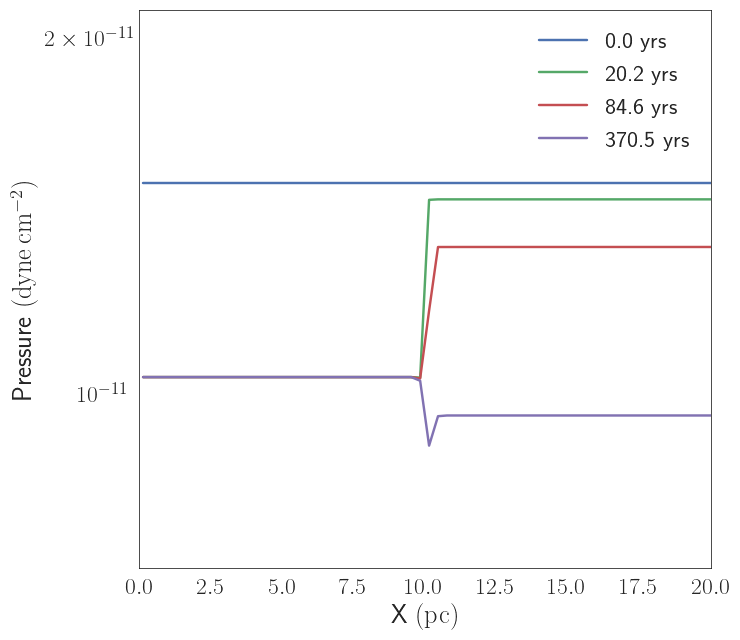
\includegraphics[width=1\linewidth]{../Document/DataImages/TabCoolingPRSprofile-micro}
			\end{center}
	\end{columns}
\end{frame}

%\begin{frame}{Σφαιρικό νέφος μέσα στο ISM}{SNEq Cooling}
%	\begin{columns}
%		\column{0.45\textwidth}
%			\begin{center}
%				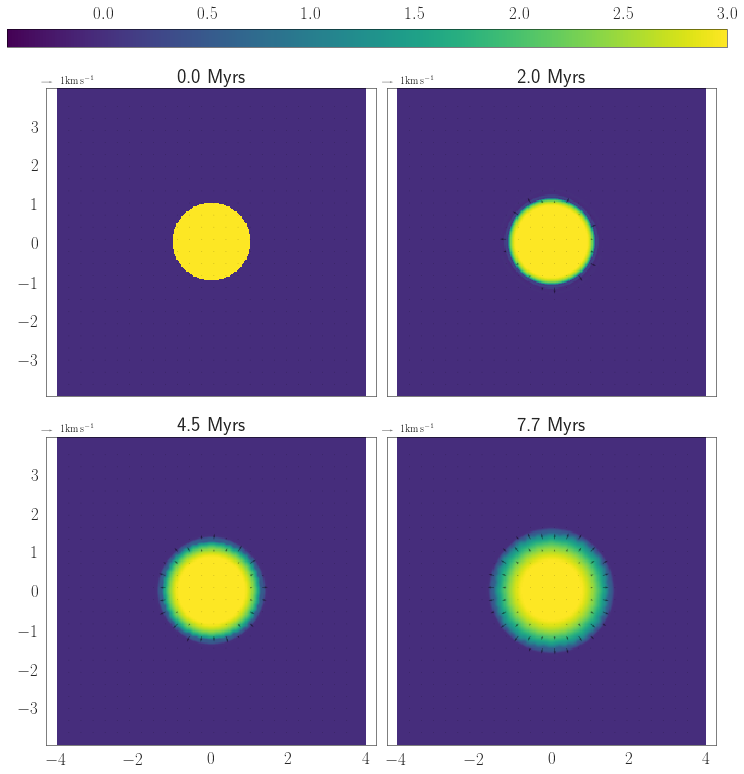
\includegraphics[width=1\linewidth]{../Document/DataImages/SNCoolingRHOquad}
%			\end{center}
%		\column{0.55\textwidth}
%			Σε κάθε βήμα της προσομοίωσης ο κώδικας ολοκληρώνει μαζί με τις υδροδυναμικές εξισώσεις και την χρονική μεταβολή του $x_{\ce{HI}}$ 
%		μαζί με την εξίσωση της ενέργειας:
%		\begin{equation}
%		\pdv{t}(\rho e)=-\Lambda=-n_e n_{\ce{H}} \left( \sum\limits_{k=1}^{16}j_k +w_{i/r} \right) 
%		\end{equation}
%		όπου η άθροιση στα $k$ υπολογίζει 16 διαφορετικές γραμμές εκπομπής.
%	\end{columns}
%%	Θεωρήσαμε σαν αρχική συνθήκη το ποσοστό του ουδετέρου υδρογόνου να είναι στο εσωτερικό του νέφους $x_{\ce{HI}}=0.1$ οπότε θα περιμέναμε λόγω της χαμηλής θερμοκρασίας και υψηλής πυκνότητας το ποσοστό αυτό να αυξηθεί. Στο εξωτερικό του νέφους, με το ίδιο σκεπτικό, χρησιμοποιούμε τη τιμή $x_{\ce{HI}}=0.9$ οπότε αντίστοιχα περιμένουμε λόγω της υψηλής θερμοκρασίας και της χαμηλής πυκνότητας σχεδόν ολόκληρο το υδρογόνου να είναι σε ατομική μορφή. 
%\end{frame}
%
%\begin{frame}{Σφαιρικό νέφος μέσα στο ISM}{SNEq Cooling}
%	\begin{center}
%		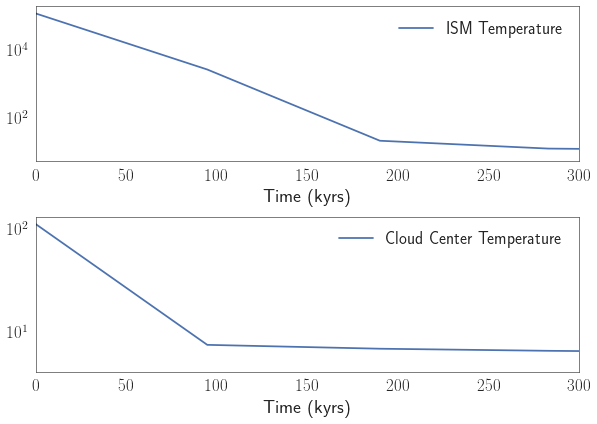
\includegraphics[width=0.9\linewidth]{../Document/DataImages/SNCoolingTMPcenterISM}
%	\end{center}
%\end{frame}
%
%\begin{frame}{Σφαιρικό νέφος μέσα στο ISM}{SNEq Cooling}
%	\begin{columns}
%		\column{0.5\textwidth}
%			\begin{center}
%				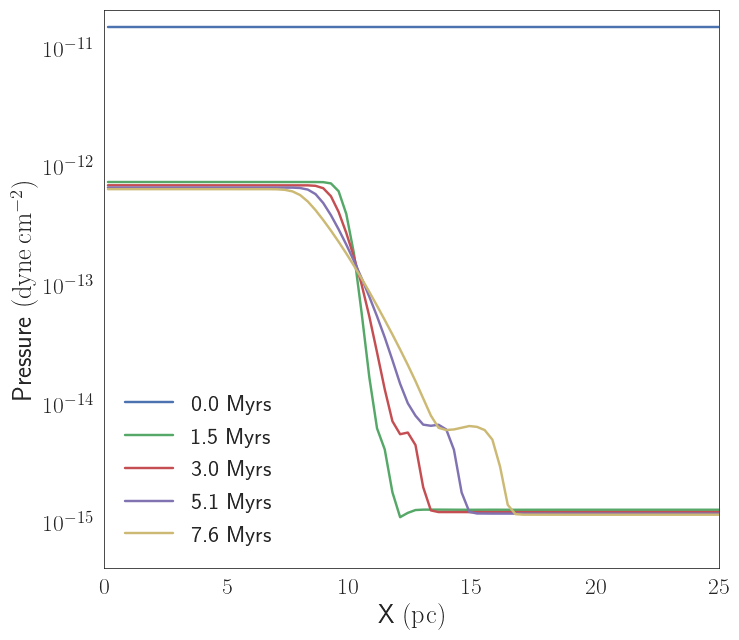
\includegraphics[width=1\linewidth]{../Document/DataImages/SNCoolingPRSprofile}
%			\end{center}
%		\column{0.5\textwidth}
%			\begin{center}
%				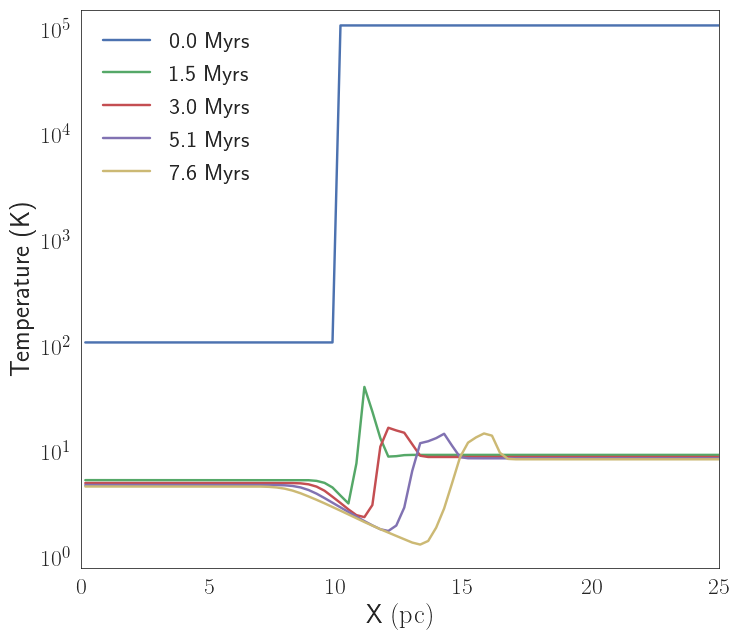
\includegraphics[width=1\linewidth]{../Document/DataImages/SNCoolingTMPprofile}
%			\end{center}
%	\end{columns}
%Λόγω της σχεδόν ισοδύναμης ψύξης του νέφους με το μεσοαστρικό περιβάλλον η διαφορά πίεσης είναι μικρότερη όπως και η ταχύτητα του ήχου στο εσωτερικό του νέφους με αποτέλεσμα η φαινομενική κατάρρευση της κεντρικής περιοχής να είναι πολύ πιο αργή σε σχέση με το Tabulated Cooling.
%\end{frame}
%
%\begin{frame}{Σφαιρικό νέφος μέσα στo ISM}{SNEq Cooling}
%	
%\begin{center}
%	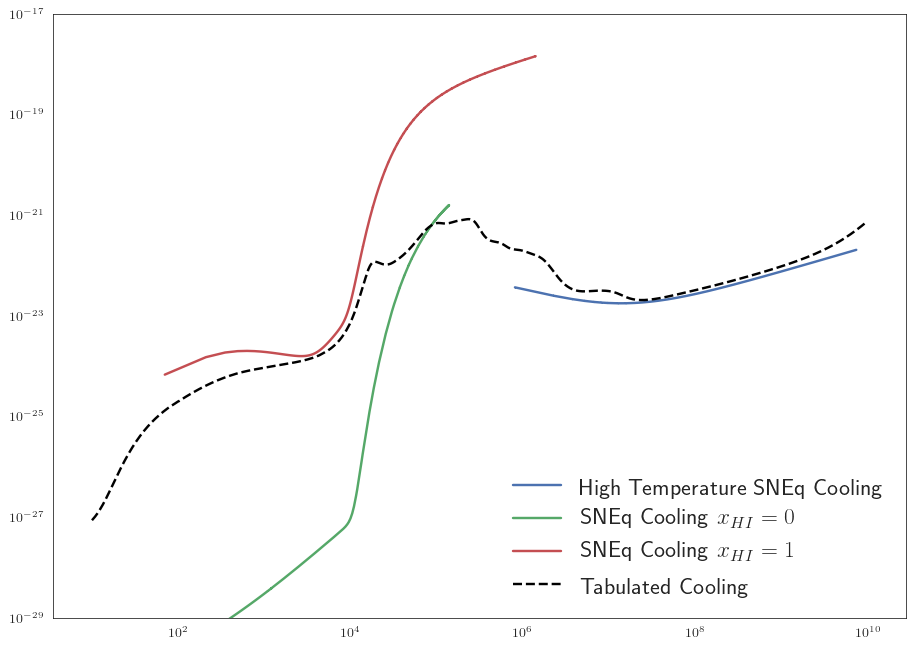
\includegraphics[width=0.85\linewidth]{../Document/DataImages/SNEQcooling-function}
%\end{center}
%\end{frame}

\begin{frame}{Σφαιρικό νέφος μέσα στo ISM}{Η2 Cooling}
	Το H2COOL εισάγει 2  μεταβλητές το ποσοστό ιονισμένου υδρογόνου $x_{\ce{HII}}$ και το ποσοστό μοριακού Υδρογόνου $x_{\ce{H2}}$.
	\begin{columns}
		\column{0.5\textwidth}
	Η χημική εξέλιξη του μοριακού, ατομικού και ιονισμένου υδρογόνου ακολουθεί τις αντιδράσεις:
		\begin{align}
		&\ce{H + e^- -> H^+ + 2e^-} \\
		&\ce{H^+ + e^- -> H + h\nu}\\
		&\ce{H_2 + e^- -> 2H + e^-} \\
		&\ce{H_2 + H -> 3H}\\
		&\ce{H_2 + H_2 -> H_2 + 2H} \\
		&\ce{H + H ->[\mathtt{dust}] H_2}
		\end{align}
		\column{0.5\textwidth}
%			Ο κώδικας ολοκληρώνει τα ποσοστά των 3 ειδών υδρογόνου μέσω της επίλυσης της παραπάνω εξίσωσης μαζί με την εξίσωση μεταφοράς:
%		\begin{equation}
%		\pdv{X_i}{t}=-\va{u}\cdot \grad{X_i}+S_i
%		\end{equation}
	
		Οι ενεργειακές απώλειες λόγω ψύξης τελικά υπολογίζονται, εκτός από τις παραπάνω αντιδράσεις, από τις απώλειες ιονισμού λόγω κρούσης $\Lambda _{\mathtt{CI}}$ και επανασύνδεσης λόγω ακτινοβολίας $\Lambda _{\mathtt{RR}}$, απώλειες λόγω περιστροφής και ταλάντωσης $\Lambda _{\mathtt{rotvib}}$ και διάσπασης  $\Lambda _{\mathtt{diss}}$ των μορίων \ce{H_2}, και της διαδικασίας αλληλεπίδρασης σκόνης-αερίου $\Lambda _{\mathtt{grain}}$.
		\begin{equation}
		\Lambda = \Lambda _{\mathtt{CI}} + \Lambda _{\mathtt{RR}} +\Lambda _{\mathtt{rotvib}} + \Lambda _{\mathtt{diss}} + \Lambda _{\mathtt{grain}}
		\end{equation}
	\end{columns}
\end{frame}

\begin{frame}{Σφαιρικό νέφος μέσα στo ISM}{Η2 Cooling}
			\begin{center}
				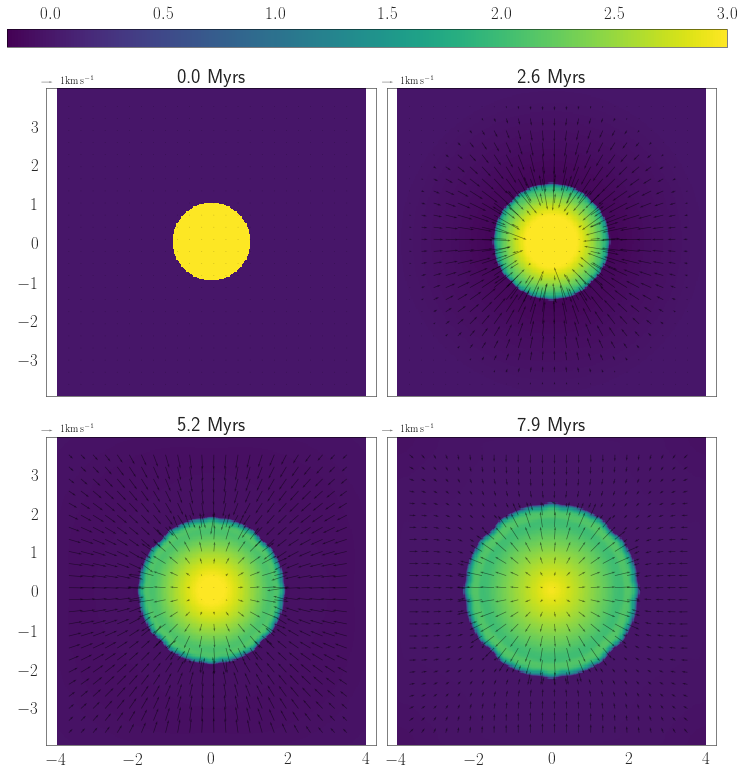
\includegraphics[width=0.6\linewidth]{../Document/DataImages/H2CoolingRHOquad}
			\end{center}

\end{frame}

\begin{frame}{Σφαιρικό νέφος μέσα στo ISM}{Η2 Cooling}
	\begin{center}
		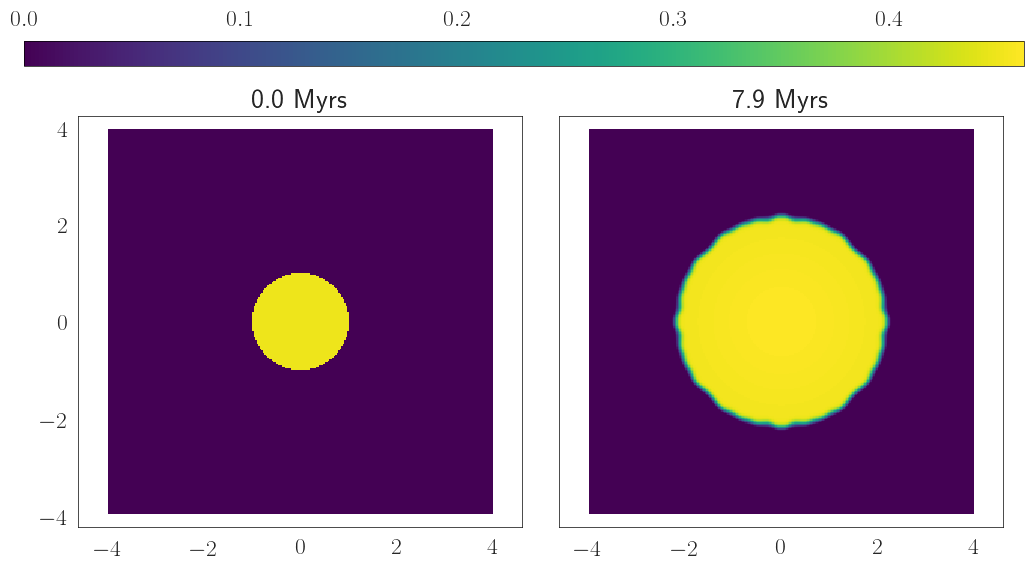
\includegraphics[height=0.25\textheight]{../Document/DataImages/H2CoolingH2quad}
	\end{center}
	\begin{center}
		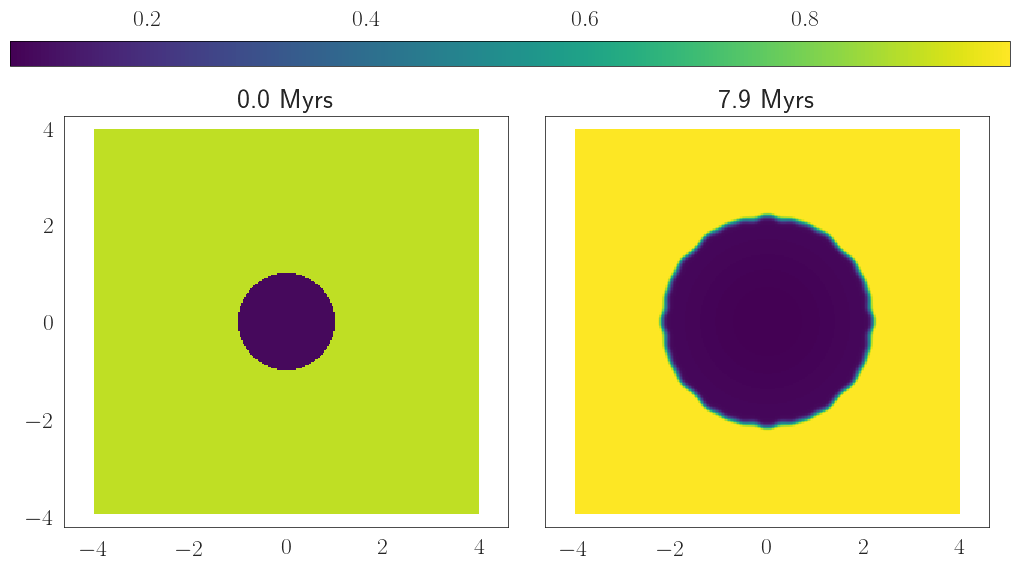
\includegraphics[height=0.25\textheight]{../Document/DataImages/H2CoolingHIquad}
	\end{center}
	\begin{center}
		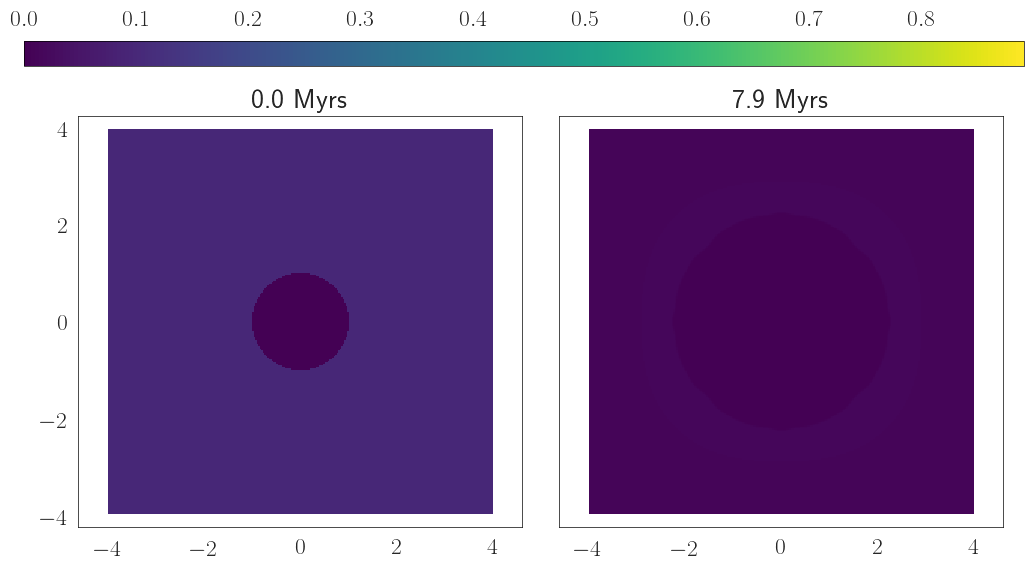
\includegraphics[height=0.25\textheight]{../Document/DataImages/H2CoolingHIIquad}
	\end{center}
\end{frame}

\begin{frame}{Σφαιρικό νέφος μέσα στo ISM}{Η2 Cooling}
	\begin{columns}
		\column{0.5\textwidth}
		
		\begin{center}
			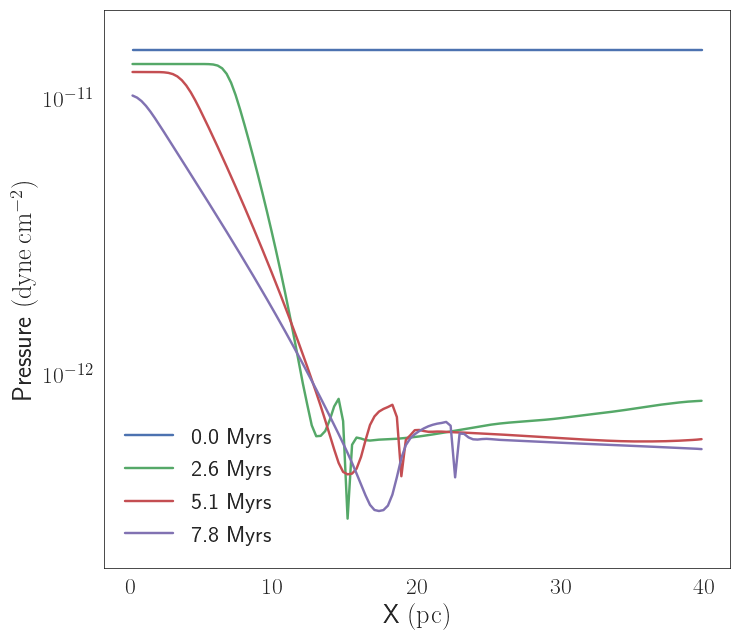
\includegraphics[width=1\linewidth]{../Document/DataImages/H2CoolingPRSprofile}
		\end{center}
		\column{0.5\textwidth}
\begin{center}
	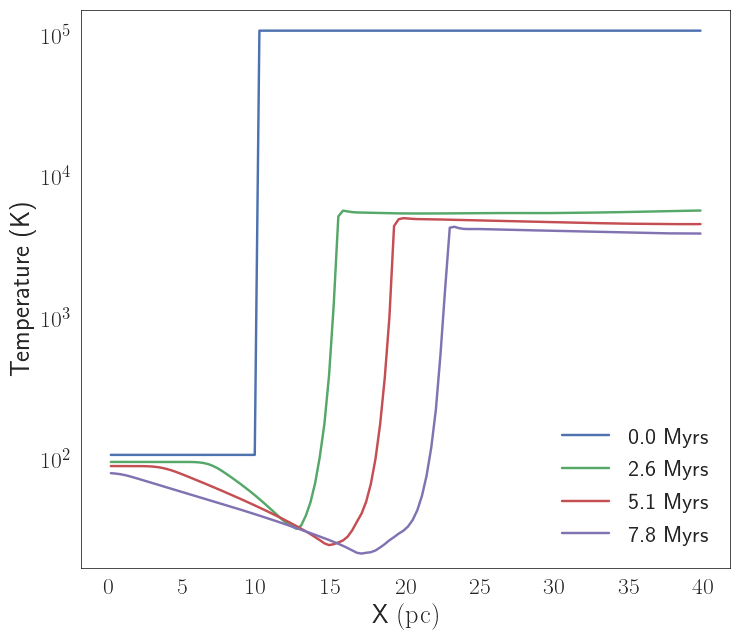
\includegraphics[width=1\linewidth]{../Document/DataImages/H2CoolingTMPprofile}
\end{center}
	\end{columns}
\end{frame}


\begin{frame}{Σφαιρικό νέφος μέσα στo ISM}{Η2 Cooling}
\begin{center}
	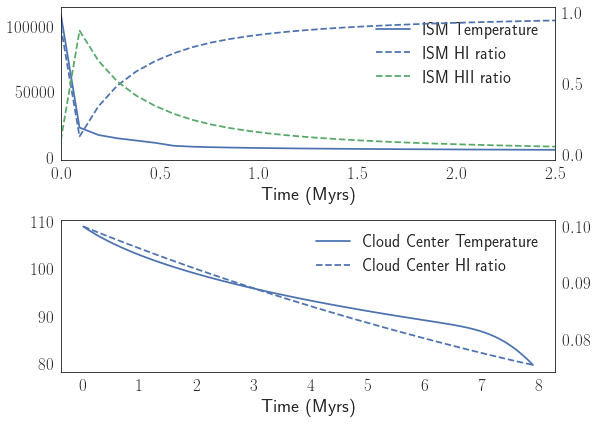
\includegraphics[width=0.8\linewidth]{../Document/DataImages/H2CoolingTMPcenterISM}
\end{center}
\end{frame}

\begin{frame}{Σφαιρικό νέφος μέσα στo ISM}{Η2 Cooling}
\begin{center}
	\includegraphics[width=0.85\linewidth]{../Document/DataImages/Η2cooling-function}
\end{center}
\end{frame}



%\begin{frame}{Cooling Functions}
%\begin{center}
%	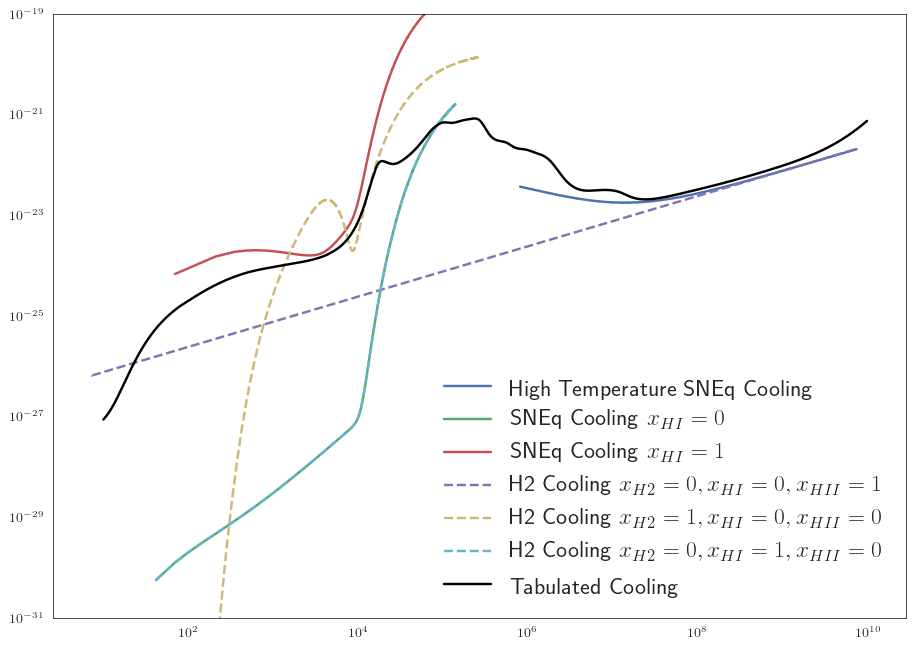
\includegraphics[width=0.8\linewidth]{../Document/DataImages/cooling-function}
%\end{center}
%\end{frame}

\begin{frame}{Σφαιρικό νέφος μέσα στo ISM}{Σύγκριση μεταξύ Tabulated και H2Cool}
	
\begin{columns}
	\column{0.5\textwidth}
	\begin{center}
		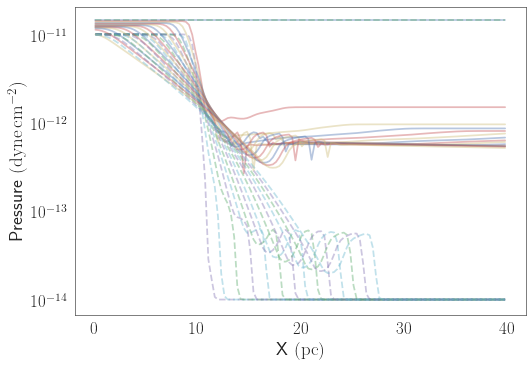
\includegraphics[width=1\linewidth]{../Document/DataImages/diffH2CoolTabCoolPRSprofile}
	\end{center}
	\column{0.5\textwidth}
\begin{center}
	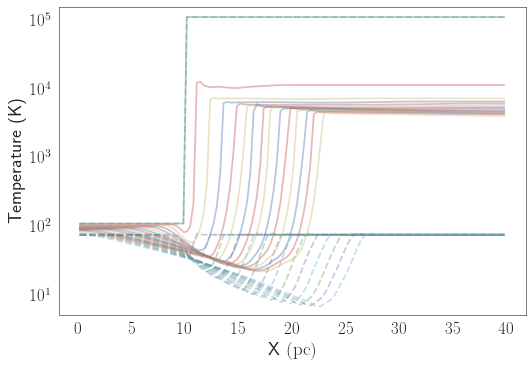
\includegraphics[width=1\linewidth]{../Document/DataImages/diffH2CoolTabCoolTMPprofile}
\end{center}
	

	
\end{columns}
\end{frame}

\begin{frame}{Βαρύτητα}%{}
	Ο PLUTO δεν μπορεί να χειριστεί την ιδιοβαρύτητα, άρα θα χρησιμοποιήσουμε τη προσέγγιση ενός ομοιογενούς βαρυτικού δυναμικού ομογενούς σφαίρας στο εσωτερικό του νέφους και ένα δυναμικό σημειακής μάζας στο εξωτερικό:
	\begin{equation}
	\vec{g}(x,y) = 
	\begin{cases}
	\frac{GM}{R^3}(x \hat{x}+ y \hat{y}) &\texttt{if } \sqrt{x^2+y^2}<R \\
	\frac{GM}{r^3}(x \hat{x}+ y \hat{y}) &\texttt{if } \sqrt{x^2+y^2}>R
	\end{cases}
	\end{equation}
		Η χρονική κλίμακα που χρειάζεται ένα σώμα να καταρρεύσει κάτω από το ίδιο το βάρος του, αν δεν υπεισέρχονται άλλες δυνάμεις ονομάζεται χρόνος ελεύθερης πτώσης:
	\begin{equation}
	t_\texttt{ff}=\sqrt{\frac{3\pi}{32G\rho}} =  \SI{1.6}{Myrs}
	\end{equation}
\end{frame}

\begin{frame}{Σφαιρικό νέφος μέσα σε βαρυτικό δυναμικό χωρίς Ψύξη}
\begin{center}
	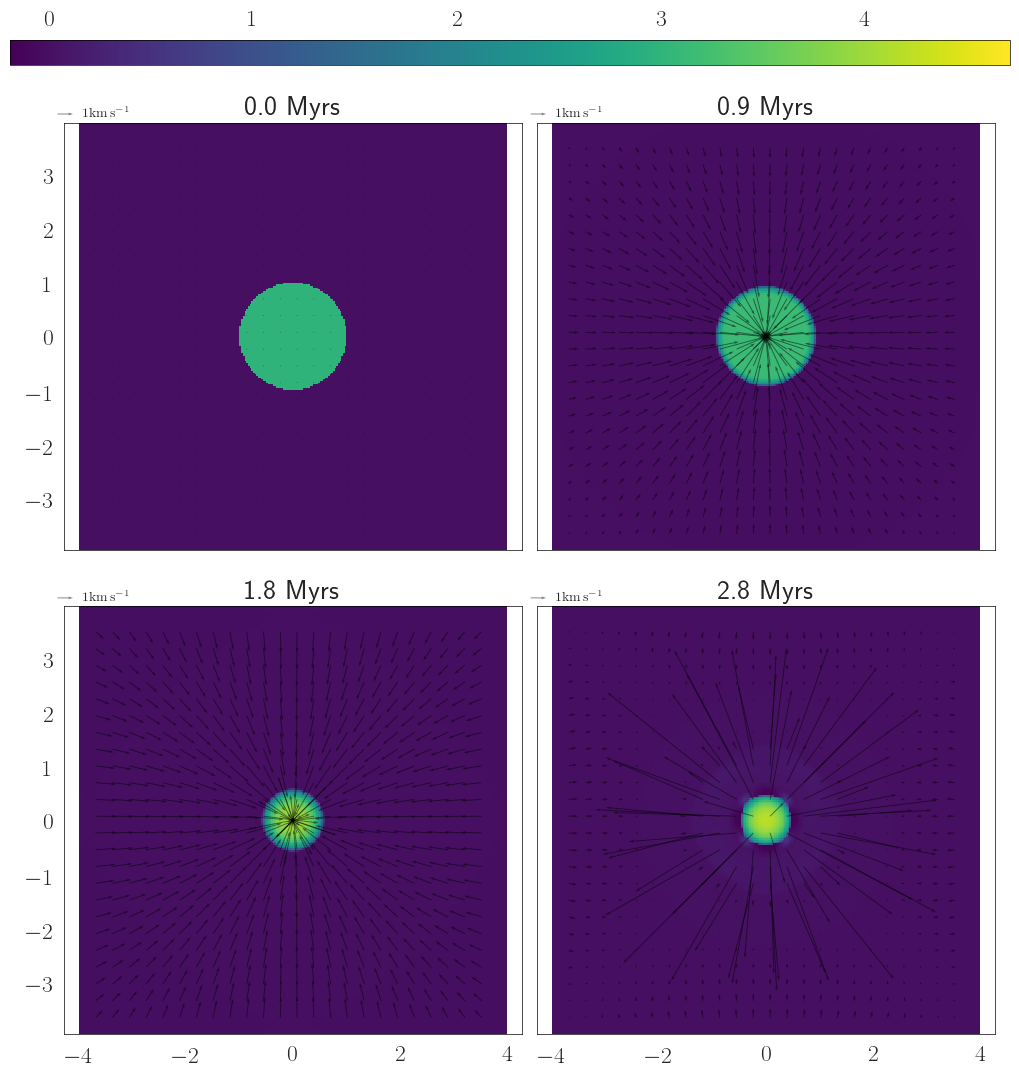
\includegraphics[width=0.6\linewidth]{../Document/DataImages/NoCoolGRquad}
\end{center}
\end{frame}

\begin{frame}{Σφαιρικό νέφος μέσα σε βαρυτικό δυναμικό χωρίς Ψύξη}{Προφίλ Πίεσης}
\begin{columns}
	\column{0.5\textwidth}
	\begin{center}
		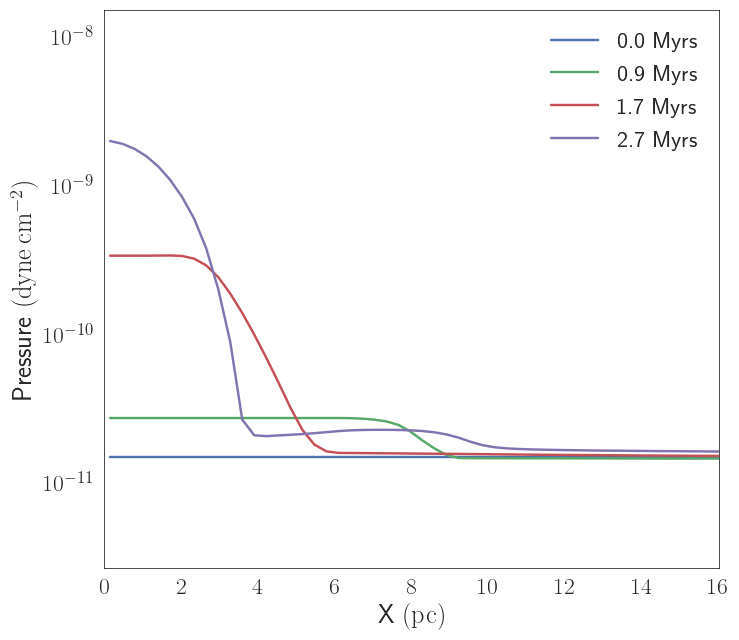
\includegraphics[width=1\linewidth]{../Document/DataImages/NoCoolGPRSprofile}
	\end{center}
	\column{0.5\textwidth}
	
\begin{center}
	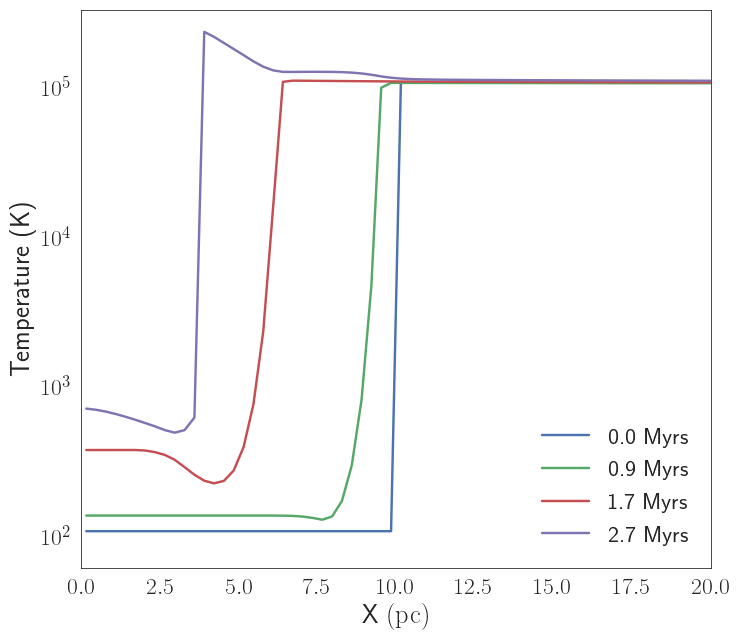
\includegraphics[width=1\linewidth]{../Document/DataImages/NoCoolGTempprofile}
\end{center}
\end{columns}
\end{frame}

\begin{frame}{Σφαιρικό νέφος σε βαρυτικό δυναμικό με Radiation Cooling}
	
	\begin{columns}
		\column{0.5\textwidth}
		\begin{center}
			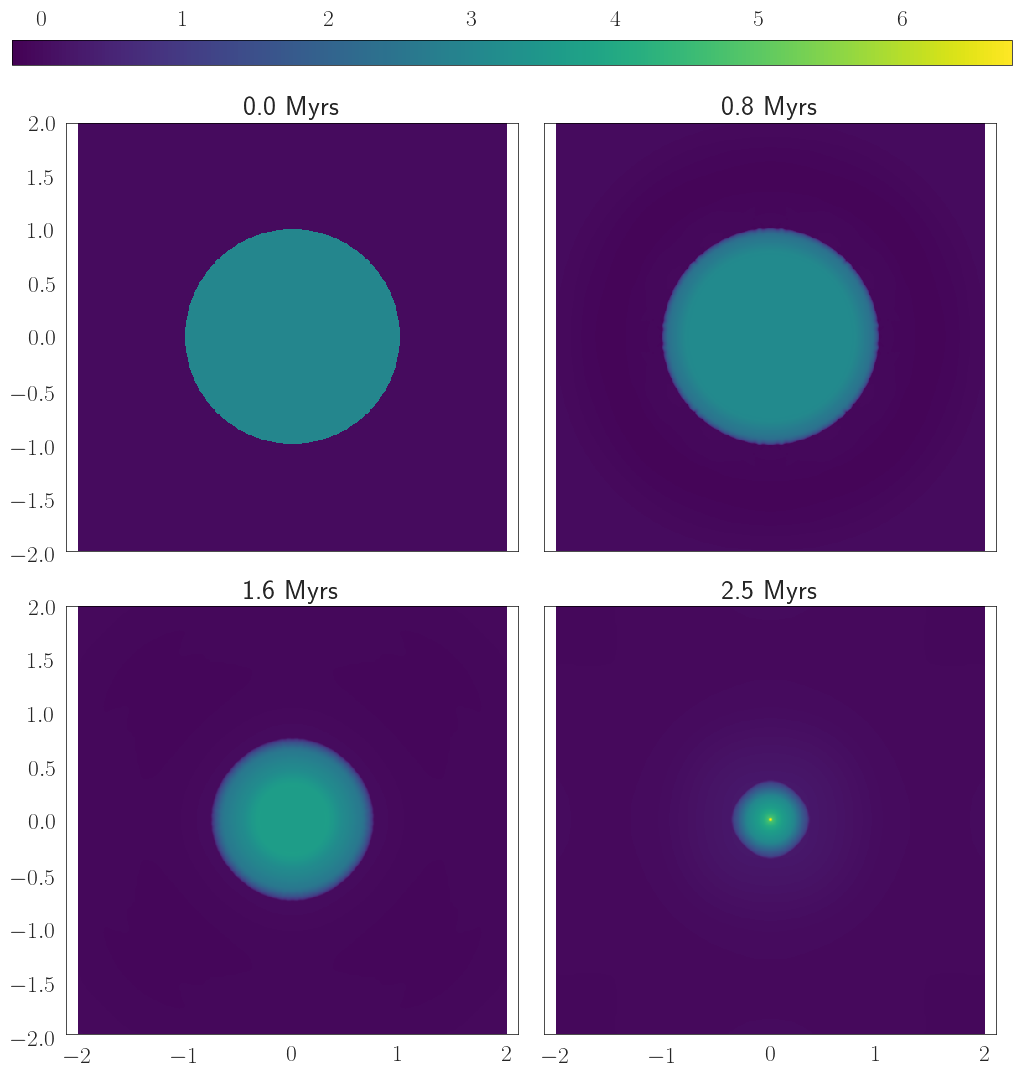
\includegraphics[width=1\linewidth]{../Document/DataImages/H2CoolGRquad}
		\end{center}
		\column{0.5\textwidth}
		Θεωρούμε σαν χρόνο κατάρρευσης το χρόνο εκείνο όπου η κεντρική περιοχή αποκτά τη μέγιστη πυκνότητα. Έτσι υπολογίζουμε 
		\begin{equation}
		t_\mathtt{col}=\SI{2.47\pm 0.05}{Myrs}
		\end{equation}
		με τη μέγιστη πυκνότητα να έχει τιμή
		\begin{equation}
		\rho _\mathtt{max}=\SI{1.29e-17}{g.cm^{-3}}
		\end{equation}
	\end{columns}
\end{frame}

\begin{frame}{Σφαίρα Bonnor - Ebert}%{}
	Οπτικά διαφανές, σφαιρικό μοριακό νέφος το οποίο βρίσκεται σε ισόθερμη κατάρρευση	
	\begin{align}
	\frac{GM_r}{r^2} +\frac{1}{\rho}\frac{dP}{dr}=0  &\qquad \text{Εξίσωση Κίνησης}\\
	\frac{dM_r}{dr} = 4 \pi r^2 \rho &\qquad \text{Εξίσωση Διατήρησης της Μάζας}\\
	P = c_s ^2 \rho &\qquad \text{Καταστατική Εξίσωση}
	\end{align}
	
	Συνδυάζοντας και τις τρεις έχουμε την εξίσωση Emden:
	\begin{equation}
	\frac{1}{r^2}\frac{d}{dr} \left( r^2 c_s ^2 \frac{d \ln \rho}{dr}\right)  = -4 \pi G \rho
	\end{equation}
	
	Θα επικεντρωθούμε στην απλούστερη λύση αυτής της εξίσωσης, όπου η κεντρική πυκνότητα είναι άπειρη (λύση SIS - Singular Isothermal Sphere):
	\begin{equation}
	\label{eq:B-E_density}
	\rho _\mathtt{BE}(r) =\frac{c_s ^2}{2 \pi G} \frac{1}{r^2}
	\end{equation}
	
\end{frame}	

\begin{frame}{Σφαιρικό νέφος σε βαρυτικό δυναμικό με Radiation Cooling}
	
\begin{center}
	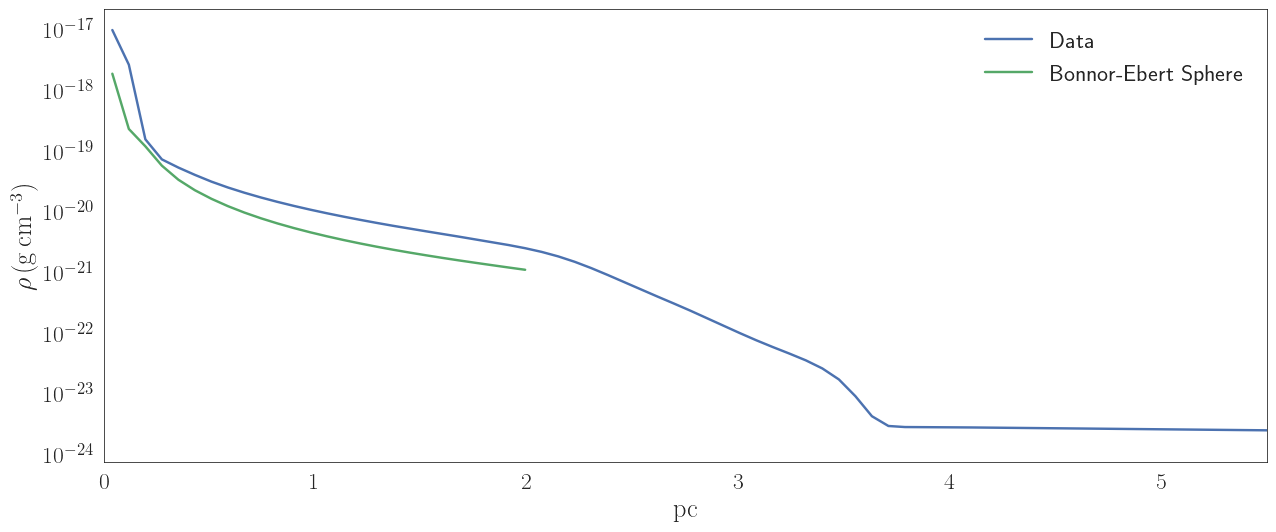
\includegraphics[width=0.8\linewidth]{../Document/DataImages/H2CoolGRHOprofile-BE}
\end{center}
\end{frame}	
	
\begin{frame}{Σφαιρικό νέφος σε βαρυτικό δυναμικό με Radiation Cooling}
	
\begin{center}
	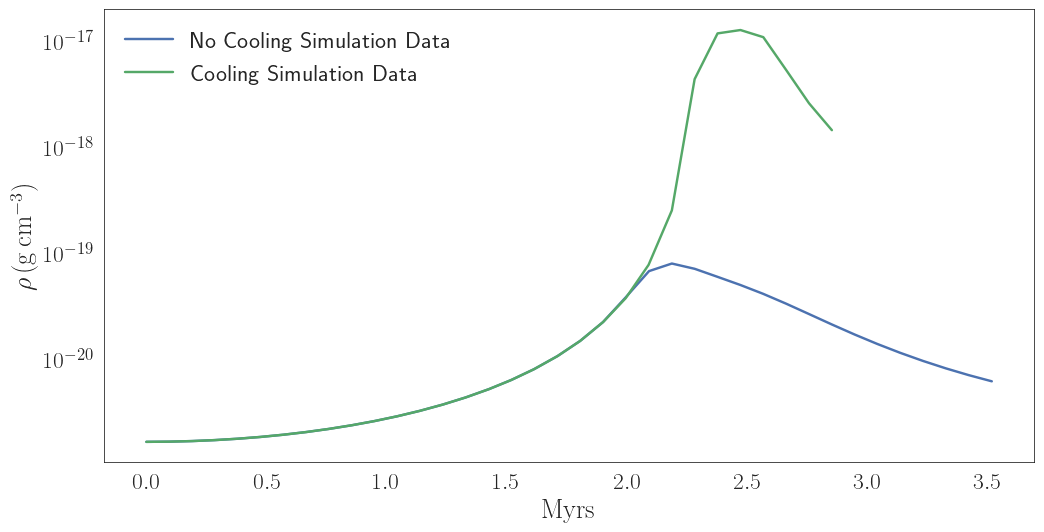
\includegraphics[height=0.4\textheight]{../Document/DataImages/GRcenterTimeRHO}
\end{center}
\begin{center}
	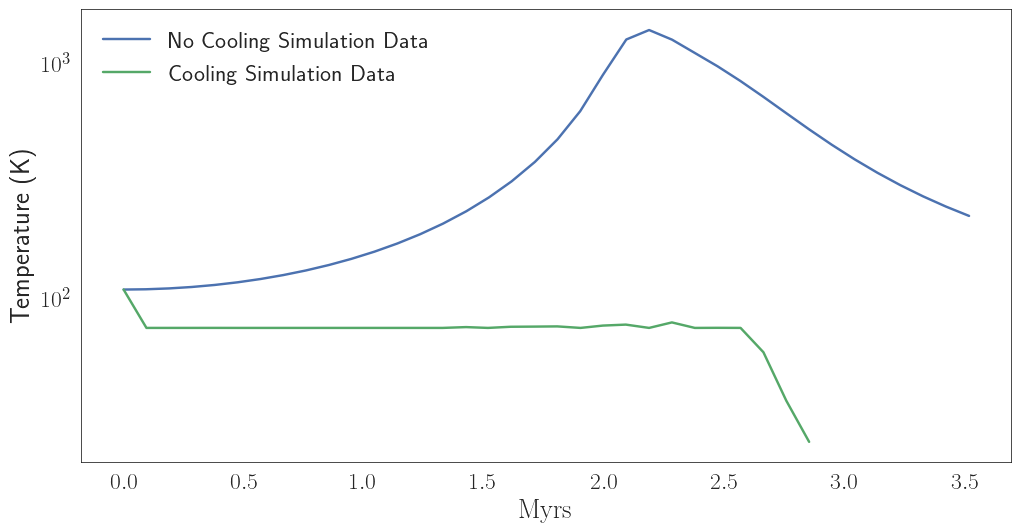
\includegraphics[height=0.4\textheight]{../Document/DataImages/GRcenterTimeTemp}
\end{center}
\end{frame}	

\begin{frame}{Δημιουργία Μοντέλου κατανομής Πυκνότητας}
	
%	 Ρεαλιστικότερες λύσεις της σφαίρας Bonnor - Ebert   προσεγγίζονται ικανοποιητικά από τη παραπάνω εξίσωση μέχρι μια κρίσιμη απόσταση $r_c=\frac{c_s}{\sqrt{4\pi G \rho _c}}$ όπου $\rho _c$ η πυκνότητα στο κέντρο $(r=0)$.
%	 
%	  Η κρίσιμη απόσταση για μια κεντρική πυκνότητα της τάξης των \SI{1e-19}{g.cm^{-3}} βρίσκεται στα περίπου \SI{0.1}{pc}. Για τη προσομοίωση μας η απόσταση αυτή αντιστοιχεί στα \SI{1.2}{pixel}, επομένως για να συγκρίνουμε επικεντρωνόμαστε στη SIS λύση.
%	 
\begin{columns}
	\column{0.5\textwidth}
	 Θα χρησιμοποιήσουμε μια κατανομή της μορφής Plummer:
	\begin{equation}
	\rho (r)=\frac{A}{B+r^a}
	\end{equation}
	όπου $A=\rho _c r_c^a$, $B=r_c^a$ με $a$ το νόμο δύναμης. 
	
	
	Από τη κατανομή που μας δίνει η προσομοίωση υπολογίζουμε μέσω της μεθόδου των ελαχίστων τετραγώνων τη τιμή για το νόμο δύναμης
	\begin{equation}
	a=\num{2.3\pm 0.14}
	\end{equation}
%	 η προσομοίωση μας δεν μπορεί να περιγράψει απόλυτα ρεαλιστικά ένα μοριακό νέφος. Γι αυτό το λόγο δεν προσπαθούμε να να προσαρμόσουμε μια -πολύπλοκη- καμπύλη πυκνοτήτων πάνω στα αποτελέσματα μας, παρά να μελετήσουμε μια γενικότερη συμπεριφορά και να κρίνουμε αν η ψύξη λειτουργεί σε ικανοποιητικό βαθμό.
	 
	\column{0.5\textwidth}
	Η εκτίμηση των υπολοίπων παραμέτρων γίνεται με βάση "εμπειρικά" δεδομένα από τα μοριακά νέφη. Για μια ακτίνα ενός μέσου μοριακού νέφους στα \SI{10}{pc} και μια συνολική μάζα τάξης \SI{1e3}{M_\odot} ταυτόχρονα με τη συνθήκη η πυκνότητα στο άκρο του νέφους να μην έχει μεγάλη διαφορά πολύ από αυτή του μεσοαστρικού αερίου βρίσκουμε
	\begin{align}
	A=10 && B=0.002
	\end{align}
	
	Έτσι υπολογίζουμε
	\begin{align}
	\rho _c = \frac{A}{B}= \SI{5000}{cm^{-3}} && r_c = B^{1/a} = \SI{0.67}{pc}
	\end{align}
\end{columns}
\end{frame}

\begin{frame}{Μοντέλο κατανομής Πυκνότητας}{Motivation}
	\begin{columns}
		\column{0.5\textwidth}
			\begin{center}
				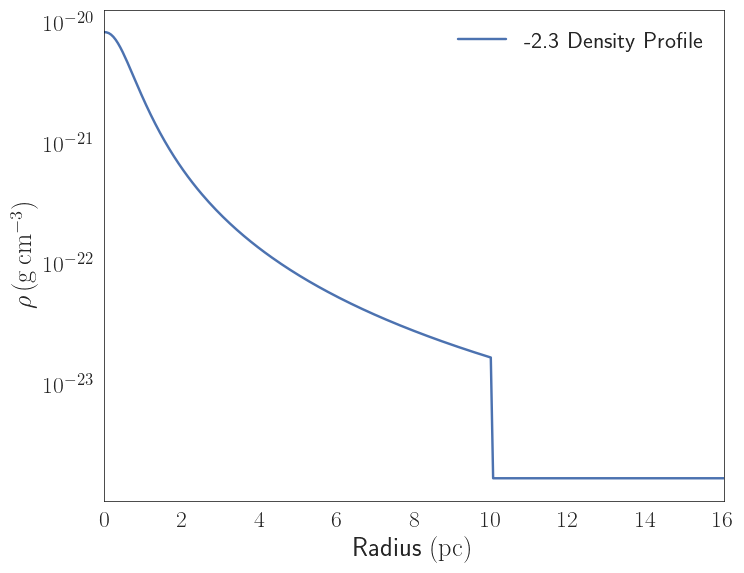
\includegraphics[width=1\linewidth]{../Document/DataImages/SimRHOProfile}
			\end{center}
		\column{0.5\textwidth}
		\begin{itemize}
			\item{Θα χρησιμοποιήσουμε το μοντέλο για τη προσομοίωση της αλληλεπίδρασης Πίδακα με Νέφος}
			\item{Η κατανομή του νέφους μένει σταθερή για χρονική κλίμακα μεγαλύτερη από το χρόνο της αλληλεπίδρασης}
		\end{itemize}
	\end{columns}
\end{frame}

\begin{frame}{Αλληλεπίδραση Σχετικιστικού Πίδακα με το ISM}
	\begin{columns}
		\column{0.5\textwidth}
		
\begin{center}
	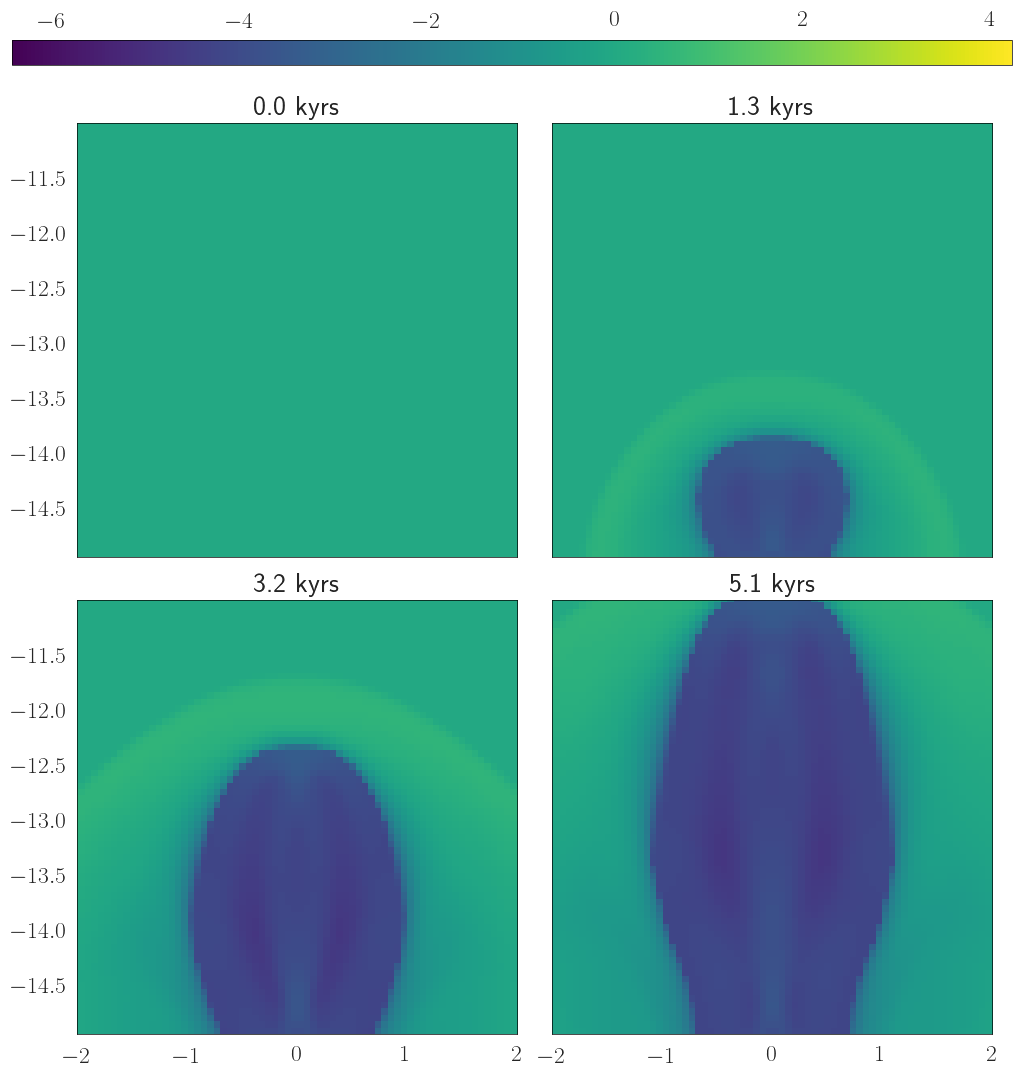
\includegraphics[width=1\linewidth]{../Document/DataImages/JetISMRHO}
\end{center}
		\column{0.5\textwidth}
		
\begin{center}
	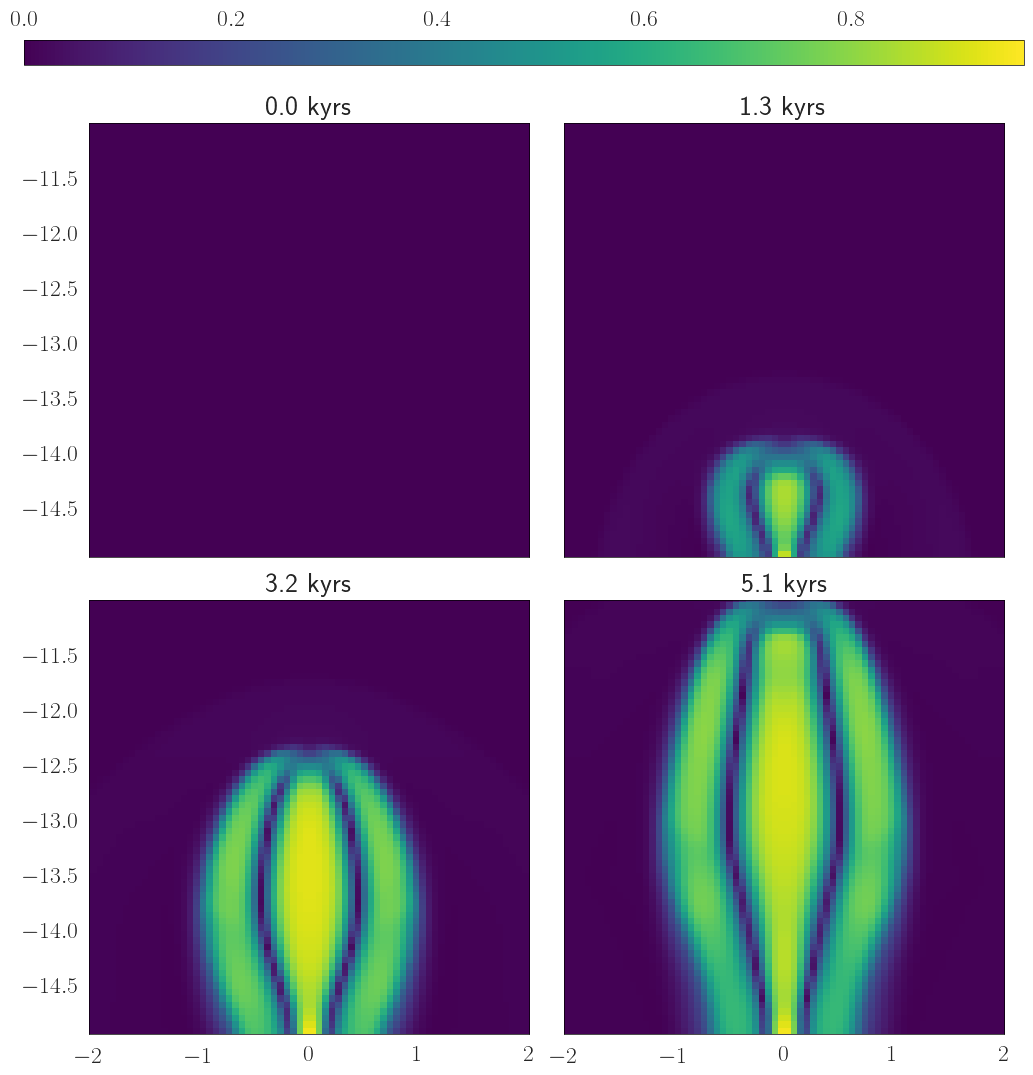
\includegraphics[width=1\linewidth]{../Document/DataImages/JetISMV}
\end{center}
	\end{columns}
\end{frame}

\begin{frame}{Αλληλεπίδραση Σχετικιστικού Πίδακα με το ISM}
	
\begin{center}
	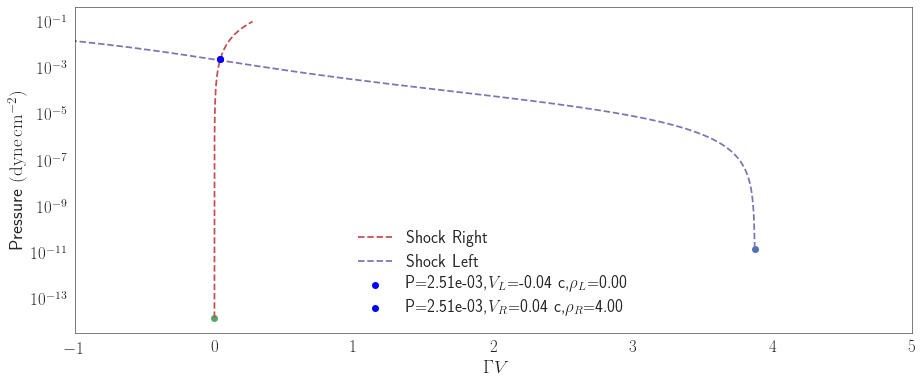
\includegraphics[width=1\linewidth]{../Document/DataImages/Shock-Shock}
\end{center}
\begin{itemize}
	\item{Συμφωνία με τη προσομοίωση}
\end{itemize}
\end{frame}


\begin{frame}%{Αλληλεπίδραση Σχετικιστικού Πίδακα με το ISM/Cloud}
	\begin{columns}
		\column{0.5\textwidth}
			\begin{center}
				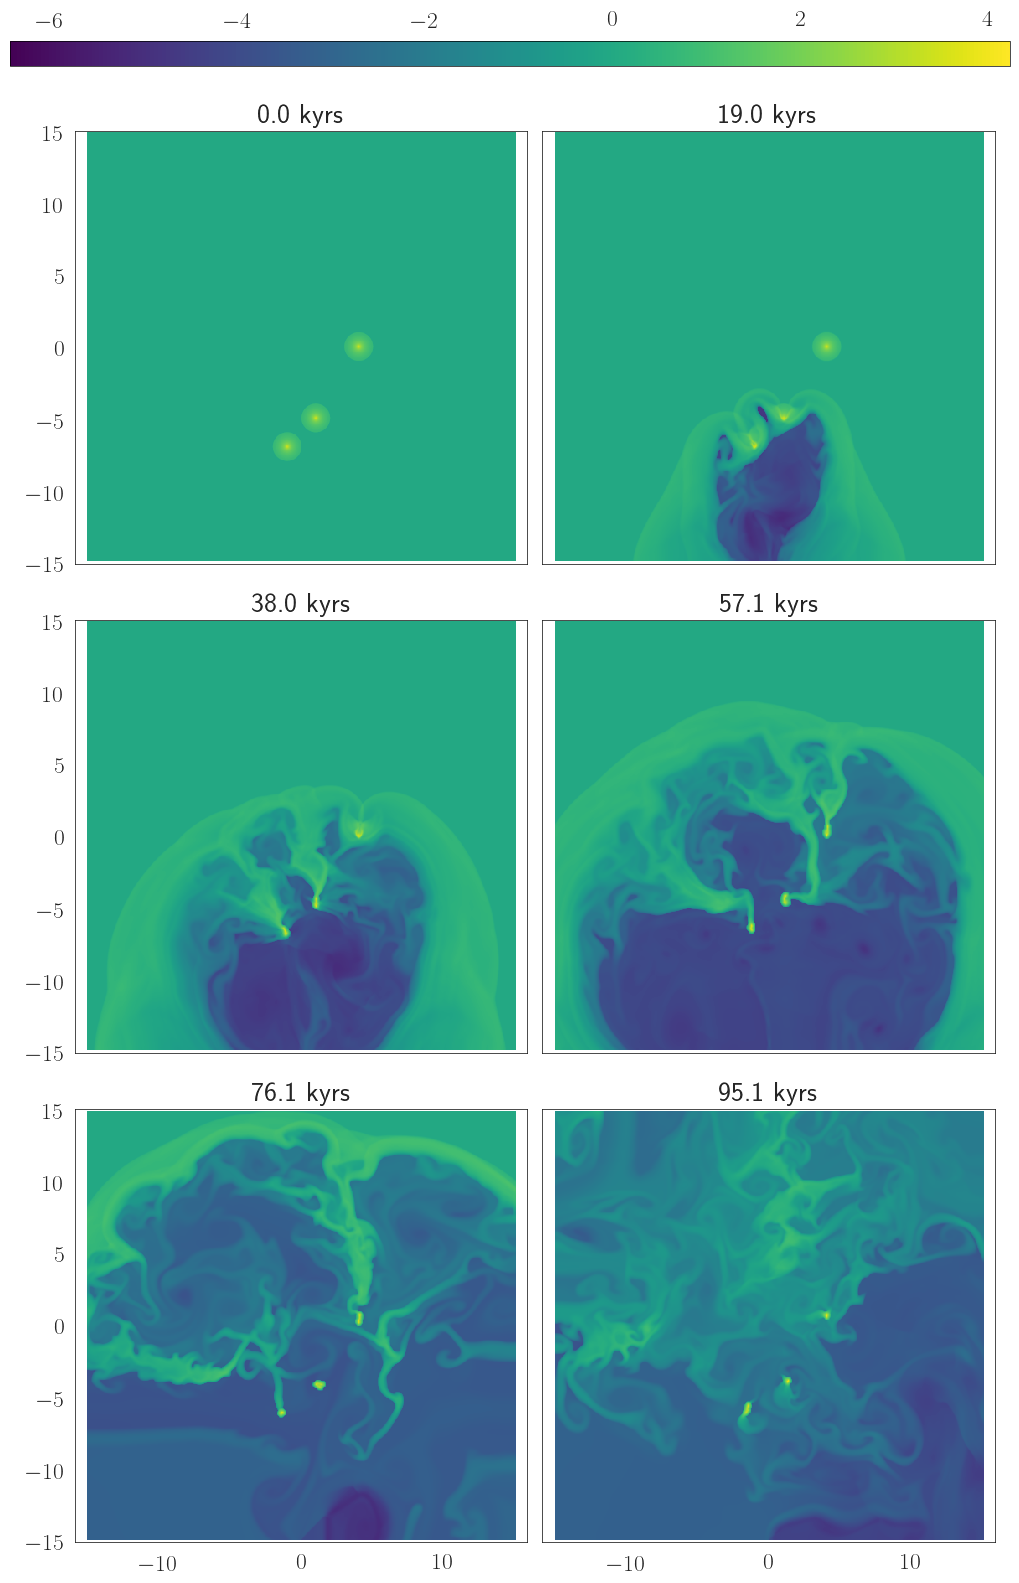
\includegraphics[width=0.925\linewidth]{../Document/DataImages/JetCloudRHO}
			\end{center}
		\column{0.5\textwidth}
			\begin{center}
				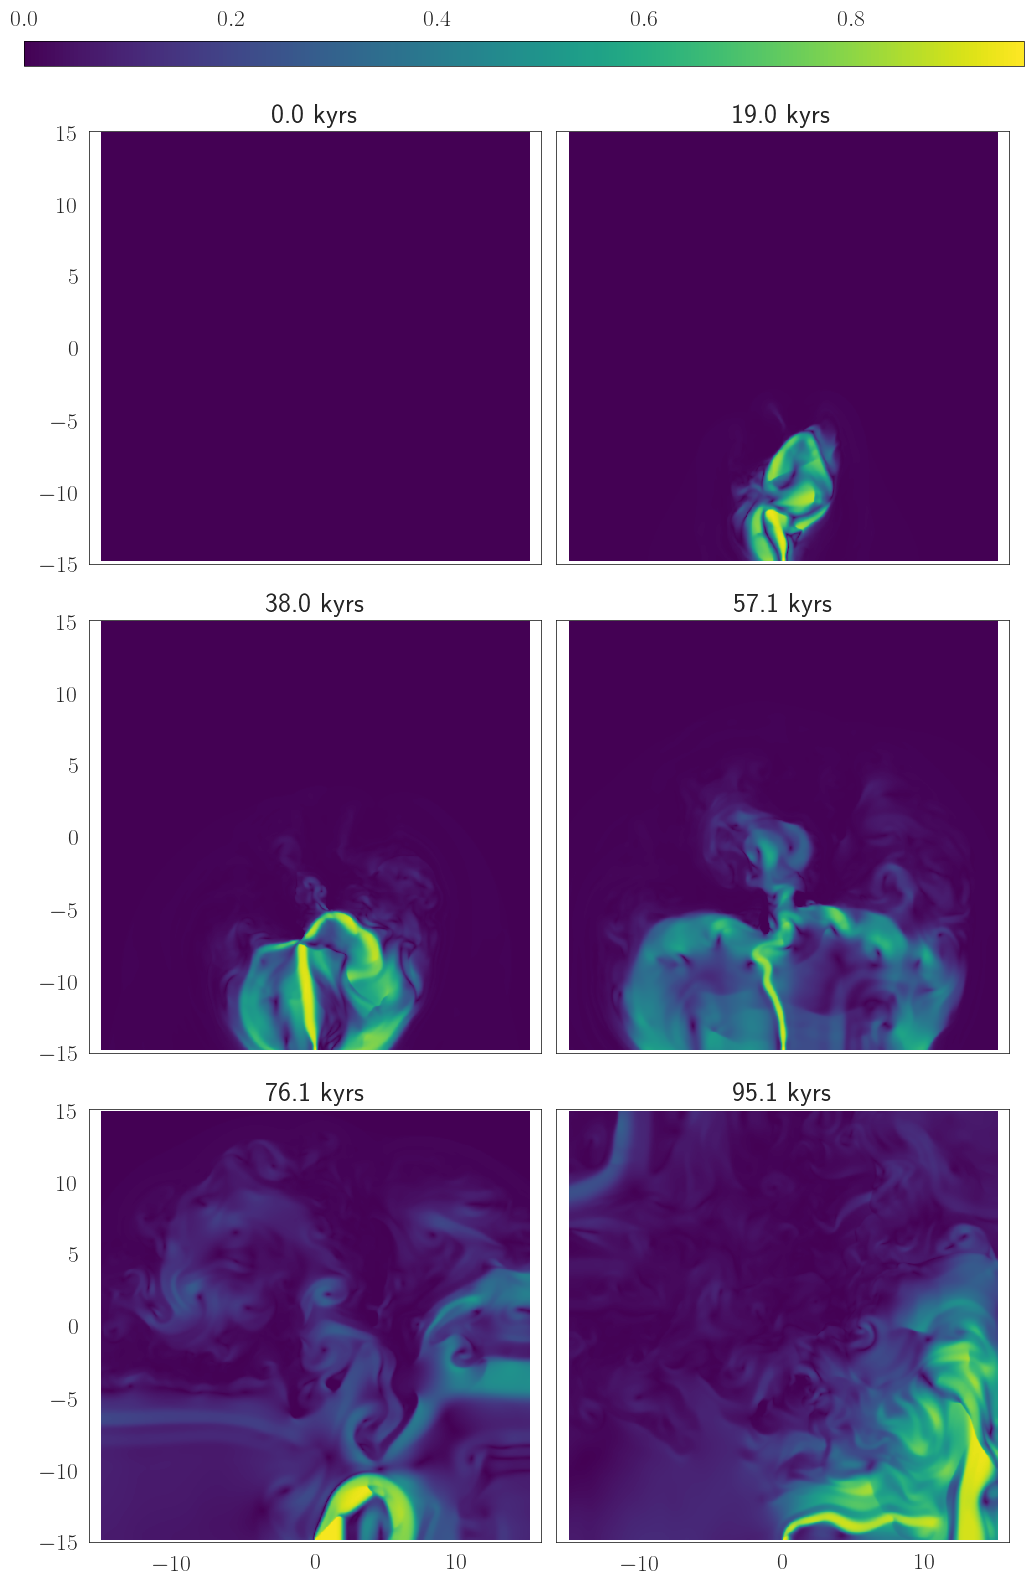
\includegraphics[width=0.925\linewidth]{../Document/DataImages/JetCloudV}
			\end{center}
	\end{columns}
\end{frame}

\begin{frame}{Αλληλεπίδραση Σχετικιστικού Πίδακα με το ISM/Cloud}
	
\begin{center}
	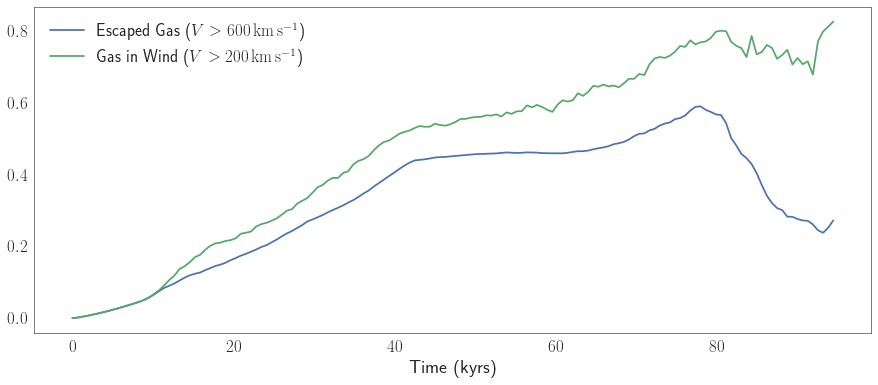
\includegraphics[width=1\linewidth]{../Document/DataImages/RatioEscapedGas}
\end{center}
Το μεγάλο ποσοστό υψηλών ταχυτήτων συμφωνεί με αντίστοιχες large-scale προσομοιώσεις (Wagner, Bicknell (2011))
\begin{itemize}
	\item{Η προσομοίωση είναι 2D}
	\item{Δεν έχουμε λάβει υπόψιν την επίδραση των μαγνητικών πεδίων}
	\item{Επίδραση από τα Boundaries}
\end{itemize}
\end{frame}

\begin{frame}{Αλληλεπίδραση Σχετικιστικού Πίδακα με το ISM }{Σύγκριση με παρατηρήσεις}
	
\begin{center}
	\includegraphics[width=1\linewidth]{Images/thejetofabla}
\end{center}
\end{frame}

\begin{frame}{Συμπεράσματα/Μελλοντική δουλειά}
	\begin{itemize}
		\item{Παρά τη χαμηλη υπολογιστική ισχύ και τις μικρές δυνατότητες που μας έδωσε ο Pluto τα αποτελέσματα ήταν ικανοποιητικά}
		\item{ARES}
		\item{Cooling Function H2}
	\end{itemize}
\end{frame}
	
%	Ρεαλιστικότερες λύσεις - χωρίς ασυνέχειες στο κέντρο της σφαίρας - προσεγγίζονται ικανοποιητικά με τη παραπάνω εξίσωση μέχρι μια κρίσιμη απόσταση $r_c=\frac{c_s}{\sqrt{4\pi G \rho _c}}$ όπου $\rho _c$ η πυκνότητα στο κέντρο $(r=0)$.  Η θεωρητική αυτή κατανομή πυκνοτήτων ονομάζεται σφαίρα Bonnor - Ebert.



%\section{Second Main Section}
%
%\subsection{Another Subsection}
%
%\begin{frame}{Blocks}
%\begin{block}{Block Title}
%You can also highlight sections of your presentation in a block, with it's own title
%\end{block}
%\begin{theorem}
%There are separate environments for theorems, examples, definitions and proofs.
%\end{theorem}
%\begin{example}
%Here is an example of an example block.
%\end{example}
%\end{frame}
%
%% Placing a * after \section means it will not show in the
%% outline or table of contents.
%\section*{Summary}
%
%\begin{frame}{Summary}
%  \begin{itemize}
%  \item
%    The \alert{first main message} of your talk in one or two lines.
%  \item
%    The \alert{second main message} of your talk in one or two lines.
%  \item
%    Perhaps a \alert{third message}, but not more than that.
%  \end{itemize}
%  
%  \begin{itemize}
%  \item
%    Outlook
%    \begin{itemize}
%    \item
%      Something you haven't solved.
%    \item
%      Something else you haven't solved.
%    \end{itemize}
%  \end{itemize}
%\end{frame}
%
%
%
%% All of the following is optional and typically not needed. 
%\appendix
%\section<presentation>*{\appendixname}
%\subsection<presentation>*{For Further Reading}
%
%\begin{frame}[allowframebreaks]
%  \frametitle<presentation>{For Further Reading}
%    
%  \begin{thebibliography}{10}
%    
%  \beamertemplatebookbibitems
%  % Start with overview books.
%
%  \bibitem{Author1990}
%    A.~Author.
%    \newblock {\em Handbook of Everything}.
%    \newblock Some Press, 1990.
% 
%    
%  \beamertemplatearticlebibitems
%  % Followed by interesting articles. Keep the list short. 
%
%  \bibitem{Someone2000}
%    S.~Someone.
%    \newblock On this and that.
%    \newblock {\em Journal of This and That}, 2(1):50--100,
%    2000.
%  \end{thebibliography}
%\end{frame}

\end{document}


